\section{Evaluation der Methode an Beispielen}\label{MFEMEvaluation}

In diesem Kapitel soll die Anwendbarkeit und Wirksamkeit von \ac{MFEM} untersucht werden. Hierzu wird die Methode an 2 Beispielen durchgeführt und anschließend ausgewertet. Es werden sämtliche Phase exemplarisch durchlaufen, dokumentiert und kurz resümiert. Zudem wird für die Durchführung der 2 Beispiele der Zeitaufwand gemessen, um auch eine Aussage über die Anwendungsdauer zu treffen. Diese spielt eine Rolle für die Akzeptanz der Methode, da eine lange Laufzeit dem Nutzen entgegensteht.\\ 
Als Ergebnis der Evaluation wird sich zeigen, ob die Methode möglichst viele Seiten eines Frameworks betrachtet und dabei repräsentative Resultate liefert.  
Um dies zu gewährleisten, müssen die richtigen Kandidaten gewählt werden.

\subsection{Wahl der Kandidaten}

Um mit der Evaluation von \ac{MFEM} möglichst vertretbare Ergebnisse zu erhalten, wurden folgenden Anforderungen an die Wahl der Kandidaten gestellt:

\begin{description}
	\item[Heterogenität] Da \ac{MFEM} eine sprachunabhängige Bewertungsmethode ist, sollten die Programmiersprachen andersartig sein.
	\item[Diskrepanz] Um Unterschiede in einzelnen Aspekten zu erhalten, sollte der Reifegrad bzw. Entwicklungsstand auseinandergehen.
	\item[Popularität] Die Frameworks sollten aktuell und relevant sein.
	\item[Opportunität] Der Zweck sollte nachgewiesenermaßen für den Einsatz in einer Microservice Architektur sein.
\end{description}

Diesen Anforderungen folgend wurde als Erstes das auf Java basierende Spring Framework\footnote{\url{spring.io}} gewählt. Es befindet sich seit 2002 in Entwicklung und hat seit dem mehrere Preise gewonnen\cite[1]{Gutierrez2016}. Dabei entwickelt es die sehr aktive Open-Source-Community ständig weiter und integriert die neuesten Technologien. Beispiele hierfür sind WebFlux, welches reaktive Webapplikationen ermöglicht, oder Cloud-Contract, um die \ac{REST}-Schnittstelle mit einem Consumer-Driven Contract abzusichern. Zudem findet jährlich die SpringOne Konferenz statt, welche mit über 2000 Teilnehmern und 30 großen Sponsoren für den Erfolg von Spring sprechen\cite{SpringOne2016}.\\
2014 wurde die Erweiterung Spring Boot offiziell veröffentlicht und stellte eine große Evolution des Frameworks dar. Es nimmt dem Entwickler so viel Arbeit wie möglich ab, sodass dieser sich auf die Geschäftslogik konzentrieren kann. Dabei stellt es die Konvention über die Konfiguration und erstellt so automatisch robuste, erweiterbare und skalierbare Spring Applikationen\cite[1]{Gutierrez2016}. Dies spricht für den hohen Reifegrad und die Akzeptanz des Frameworks.\\
Nach \cite{Wolff2016} ist das Spring Framework eine sehr gute Wahl für den Einsatz in einer Microservice Architektur und lässt dabei kaum ein Problem offen, für das es keine Lösung vorhält. 

Die Wahl des zweiten Frameworks fiel auf Go-Kit\footnote{\url{gokit.io}}. Es wird seit 2016 entwickelt und ist somit, im Gegensatz zu Spring, ein sehr junges Framework. Dabei setzen die Entwickler auf die Programmiersprache Go, welche selbst noch relativ jung ist. \\
Go wurde ursprünglich 2007 von Mitarbeitern des Unternehmens Google\cite{Golang2009} entwickelt und ist seit 2012 in einer stabilen Version verfügbar. Seit dem ist das Interesse für diese Sprache immens gestiegen, was der Tiobe Index deutlich zeigt. Dies ist ein Popularitäts-Ranking von Programmiersprachen, in dem Go derzeit den 14. Platz (Stand: Februar 2017) einnimmt\cite{Tiobe2016}. Aufgrund der starken Steigerung gegenüber dem Vorjahr wurde Go von Tiobe auch zur Programmiersprache 2016 gewählt.\\
Da Go bereits im Hinblick auf skalierbare Netzwerkdienste, Cluster- und Cloud Computing entwickelt wurde, bringt die Sprache sehr viel für die Erstellung von verteilten Systemen mit. In Bezug auf eine Microservice Architektur fehlen jedoch einige Funktionen wie z.~B. Infrastrukturintegration oder Logging. Diese Lücke versucht Go-Kit zu schließen, damit der Entwickler sich auf die Geschäftslogik konzentrieren kann.

Mit Spring und Go-Kit für die Evaluation von \ac{MFEM} werden die Anforderungen nach Heterogenität, Diskrepanz, Popularität und Opportunität erfüllt. Neben den unterschiedlichen Programmiersprachen geht der Reifegrad der Frameworks stark auseinander und sollte somit für unterschiedliche Ergebnisse sorgen. Nichtsdestotrotz erfahren 
beide aktuell einen hohen Zuspruch für den Einsatz in einer Microservice Architektur und stellen somit interessante Kandidaten dar.

\subsection{Kickoff-Phase}

Neben der Einführung der Methode sieht diese Phase eine Vorstellung der vorhandenen Microservice Architektur vor.  
Da ein Teil der Evaluation auf den in \ac{MFEM} enthaltenen Basisanforderungen und deren Wirkung liegen soll, wurde ein möglichst einfacher Entwurf der zugrundeliegenden Architektur gewählt. So ergeben sich in der Analysephase nur wenige spezifische Anforderungen, die für die Evaluation der Methode eine geringe Rolle spielen. Weitere Phasen sind von der Microservice Architektur nicht direkt betroffen und bleiben daher unberührt. Abbildung \ref{Evaluationsarchitektur} zeigt die gewählte Architektur.

\image[Evaluationsarchitektur.pdf]{Evaluationsarchitektur}{Architektur für die Evaluation}{Vorgegebene Microservice Architektur für die Evaluation}

Die Architektur teilt sich in Infrastruktur und Services auf. Services enthalten die Geschäftslogik sowie Datenhaltung. Dabei kann es verschiedene Services geben, die in mehrere Instanzen vorhanden sein können. Die genaue Form ist für die Evaluation irrelevant und wird daher nicht weiter berücksichtigt. Des Weiteren kümmert sich die Infrastruktur um den reibungslosen Ablauf und ist in Service-Discovery, Authentication-Service und API-Gateway aufgeteilt.

Das API-Gateway stellt eine einheitliche Schnittstelle des Gesamtsystems den Clients zur Verfügung. So müssen diese keine Kenntnis über die interne Struktur haben und können sämtliche Funktionen über einen zentralen Punkt nutzen. Hierzu reicht es die externen Anfragen an die jeweiligen Services weiter.

Die Service-Discovery sorgt für die Verwaltung der einzelnen Services und deren Instanzen, damit diese von anderen, z.~B. dem API-Gateway, erreicht werden können. Jede Instanz eines Services muss sich an der Discovery beim Start registrieren und einen regelmäßigen Heartbeat an diese senden. Hierzu bietet die mit Netflix Eureka erstellte Discovery eine \ac{REST}-Schnittstelle zur Verfügung. Der genaue Ablauf ist in Abbildung \ref{ServiceDiscovery} dargestellt.

\image[ServiceDiscovery.pdf][width=0.5\linewidth]{ServiceDiscovery}{Ablauf Service Discovery}{Ablauf: Zugriff über die Service Discovery}

Der Authentication Service kümmert sich um die Authentifizierung der Benutzer. Damit müssen die einzelnen Services keine eigene Benutzerverwaltung integrieren. Mit der Authentifizierung erhält der Client einen begrenzt gültigen \ac{JWT}, mit dem er auf die Services zugreifen kann. So lassen sich auch kaskadierte Anfragen realisieren, bei dem ein Service mittels des \ac{JWT} einen anderen aufruft ohne die Anmeldeinformationen des Clients zu kennen. Dies ist auch vereinfacht in Abbildung \ref{AuthFlow} dargestellt, wobei die Zwischenschritte über das API-Gateway und die Service-Discovery vernachlässigt wurden.

\image[AuthFlow.pdf][width=0.7\linewidth]{AuthFlow}{Ablauf kaskadierter Anfrage}{Vereinfachte Darstellung einer kaskadierten Anfrage eines Clients über mehrere Services}

Weitere Vorgaben über die Architektur werden nicht gemacht, da diese im Sinne der Evaluation nicht zielführend wären. Wie eingangs geschildert, würde sich dies nur in zusätzlichen Anforderungen widerspiegeln.

\subsubsection{Resümee Kickoff}

Da nur der Autor die Evaluation durchführt, gab es keine Informationen, die mit anderen Teilnehmern ausgetauscht werden mussten. Aus diesem Grund wäre diese Phase bei einer realen Anwendung übersprungen worden. Sie ist somit zu Recht nach \ac{MFEM} nur optional durchzuführen.

\subsection{Analysephase}

In der Analysephase sollen nun, mit Hilfe der gegebenen Architektur, die Anforderungen gewählt, priorisiert und um Metriken erweitert werden. Hierzu wird im nächsten Schritt ein Quality Utility Tree aufgebaut.

\subsubsection{Architektur Analyse und Wahl der Anforderungen}

Mit \ac{MFEM} kommen bereits viele die Basisanforderungen mit. Da die Architektur möglichst einfach gehalten wurde, gibt es keinen Widerspruch zu diesen Anforderungen. Auch gibt es innerhalb der Basisanforderungen keine Punkte die sich widersprechen. Sie lassen sich somit vollständig übernehmen.

Zusätzlich ergeben sich aus der Architektur funktionale Serviceanforderungen. Dies betrifft hauptsächlich die Service-Discovery. Ein Service muss sich an diesem An- und Abmelden sowie regelmäßig einen Heartbeat senden. Auch für die Inter-Service-Kommunikation muss ein Service an der Discovery die Einträge abfragen und verarbeiten können. (Abbildung \ref{ServiceDiscovery}) Somit wurde die Anforderung zur Unterstützung einer mit Eureka aufgebauten Service-Discovery aufgenommen.

In den Basisanforderungen ist bereits unter der Kategorie Sicherheit die Anforderung nach einer Absicherung gefordert. Dies beinhaltet die Unterstützung eines \ac{JWT} und wird daher nicht als eigener Punkt aufgenommen. Zusätzlich soll auf eine Autorisierung durch Benutzerrechte verzichtet werden. 
Aus diesem Grund ergeben sich durch den Authentifizierungs-Service keine weiteren Anforderungen.\\
Auch durch das Gateway ergeben sich keine Anforderungen, da die Beziehung zu den Services einseitig ist. Im vorliegenden Entwurf leitet das API-Gateway Anfragen an die Services weiter. Jedoch stellen die Services keine Anfragen an das Gateway und müssen daher keine zugehörigen Funktionen unterstützen.

Die Basisanforderungen decken bereits eine Vielzahl an nicht-funktionalen Serviceanforderungen ab. Diese beinhalten z.~B. die Forderung nach einer aktiven Community, eine effiziente Programmierung oder eine gute Dokumentation. Aus diesem Grund wird auch hier auf die Aufnahme weiterer Anforderungen verzichtet.

Nachdem alle Anforderungen zusammengetragen und in einem Quality Utility Tree eingeordnet wurden, sind diese priorisiert worden. Abbildung \ref{QUT} zeigt den entstandenen Quality Utility Tree mit allen Anforderungen für die Evaluation.

\image[QUT.pdf][width=0.9\linewidth]{QUT}{Quality Utility Tree Evaluation}{Priorisierter Quality Utility Tree mit allen Anforderungen für die Evaluation.}

\subsubsection{Metriken definieren}

Mit dem Ergebnis aus dem letzten Schritt können nun die passenden Metriken für die Anforderungen gefunden werden. \ac{MFEM} sieht hierfür den Top-Down Ansatz der \ac{GQM} Methode vor.\\
Das heißt, dass für jede Anforderungen eine oder mehrere Fragen erstellt werden, die zusammen das Ziel wiedergeben. Sie drücken somit aus, was man mit der Messung erfahren will und betrachten die Anforderung von mehreren Seiten.\\
Für alle Anforderungen wurden so Fragen erstellt und in einer Tabelle festgehalten. Darauf aufbauend wurden Metriken definiert, die die Fragen beantworten sollen.

Die gesamte in diesem Schritt erstellte Tabelle wird in \ref{GQM} dargestellt und enthält das Ergebnis der Anwendung von \ac{GQM} auf die Anforderungen mit allen definierten Metriken.  

\begin{longtable}{c}
	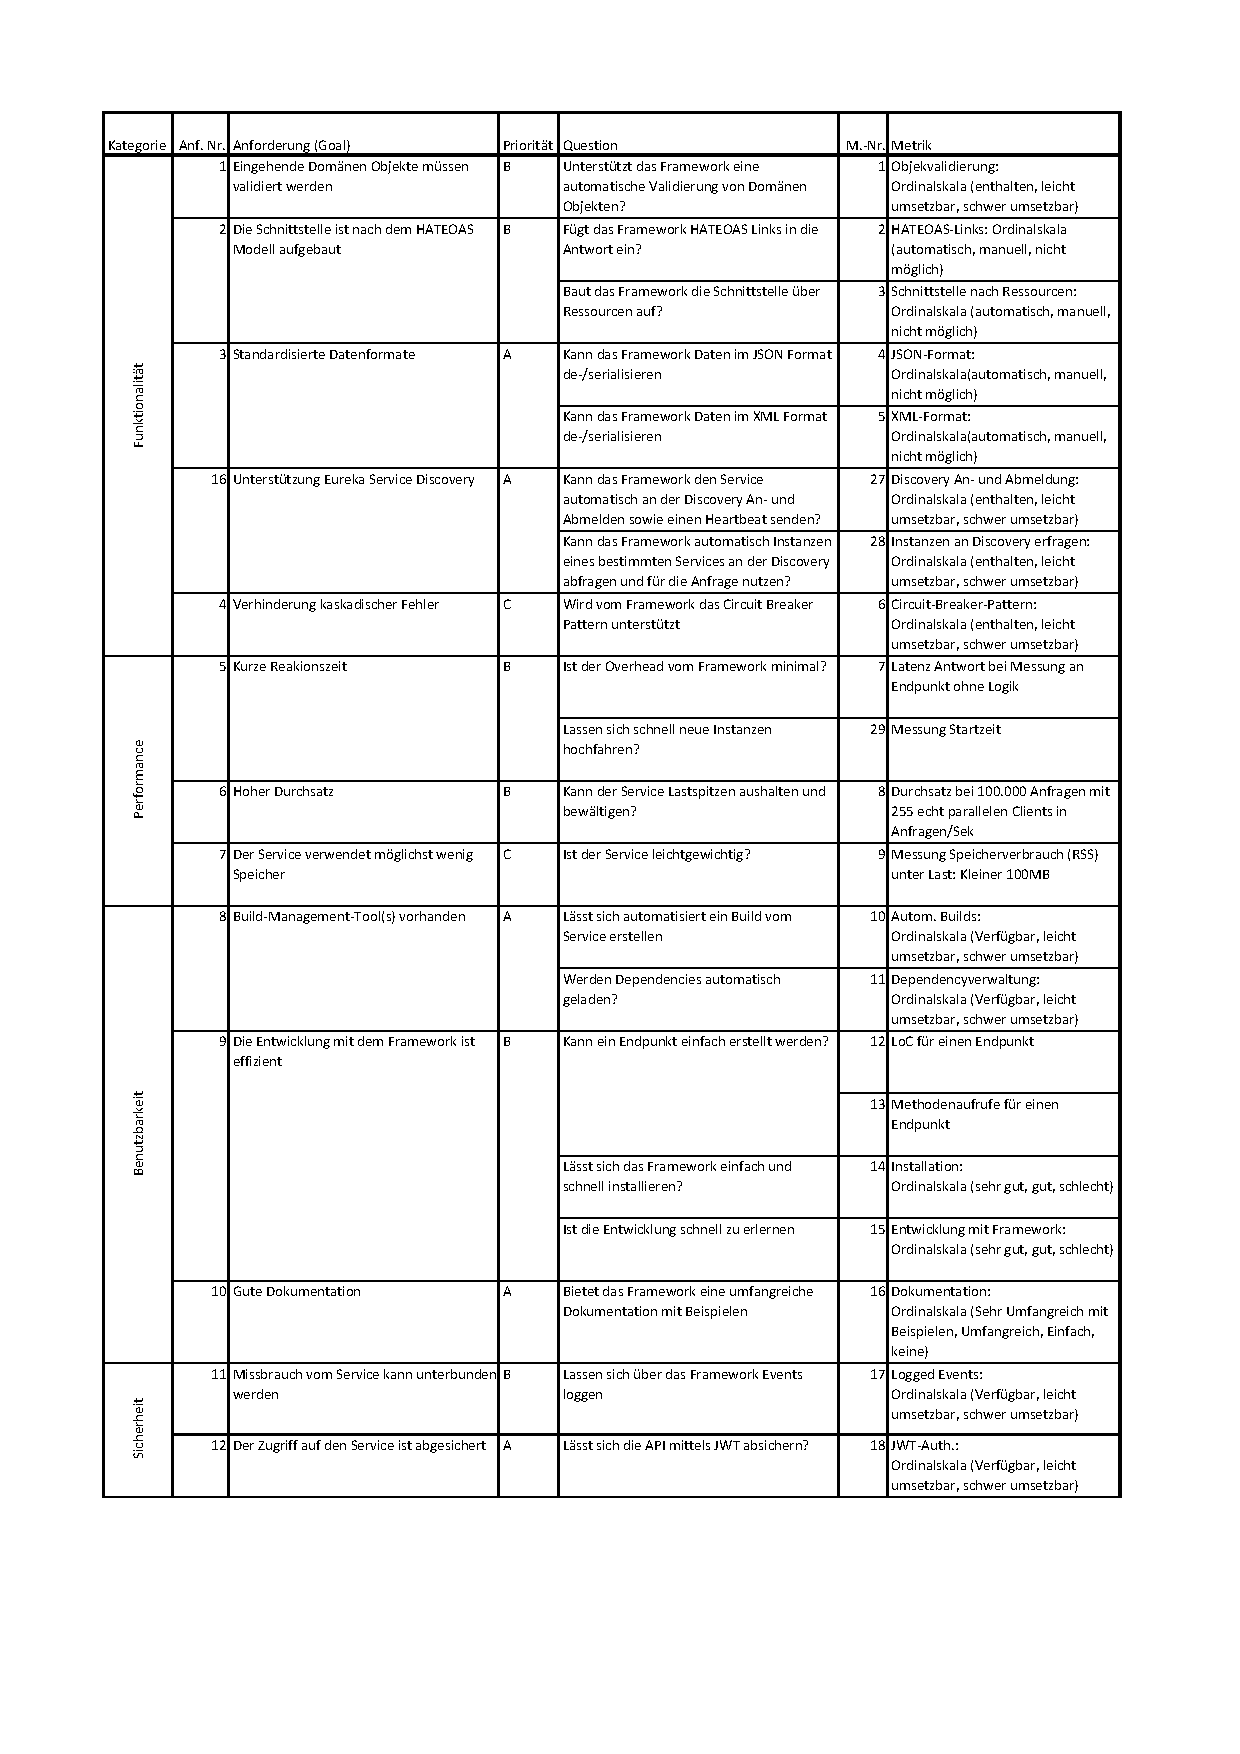
\includegraphics[width=\linewidth]{Bilder/GQM.pdf} \\	
	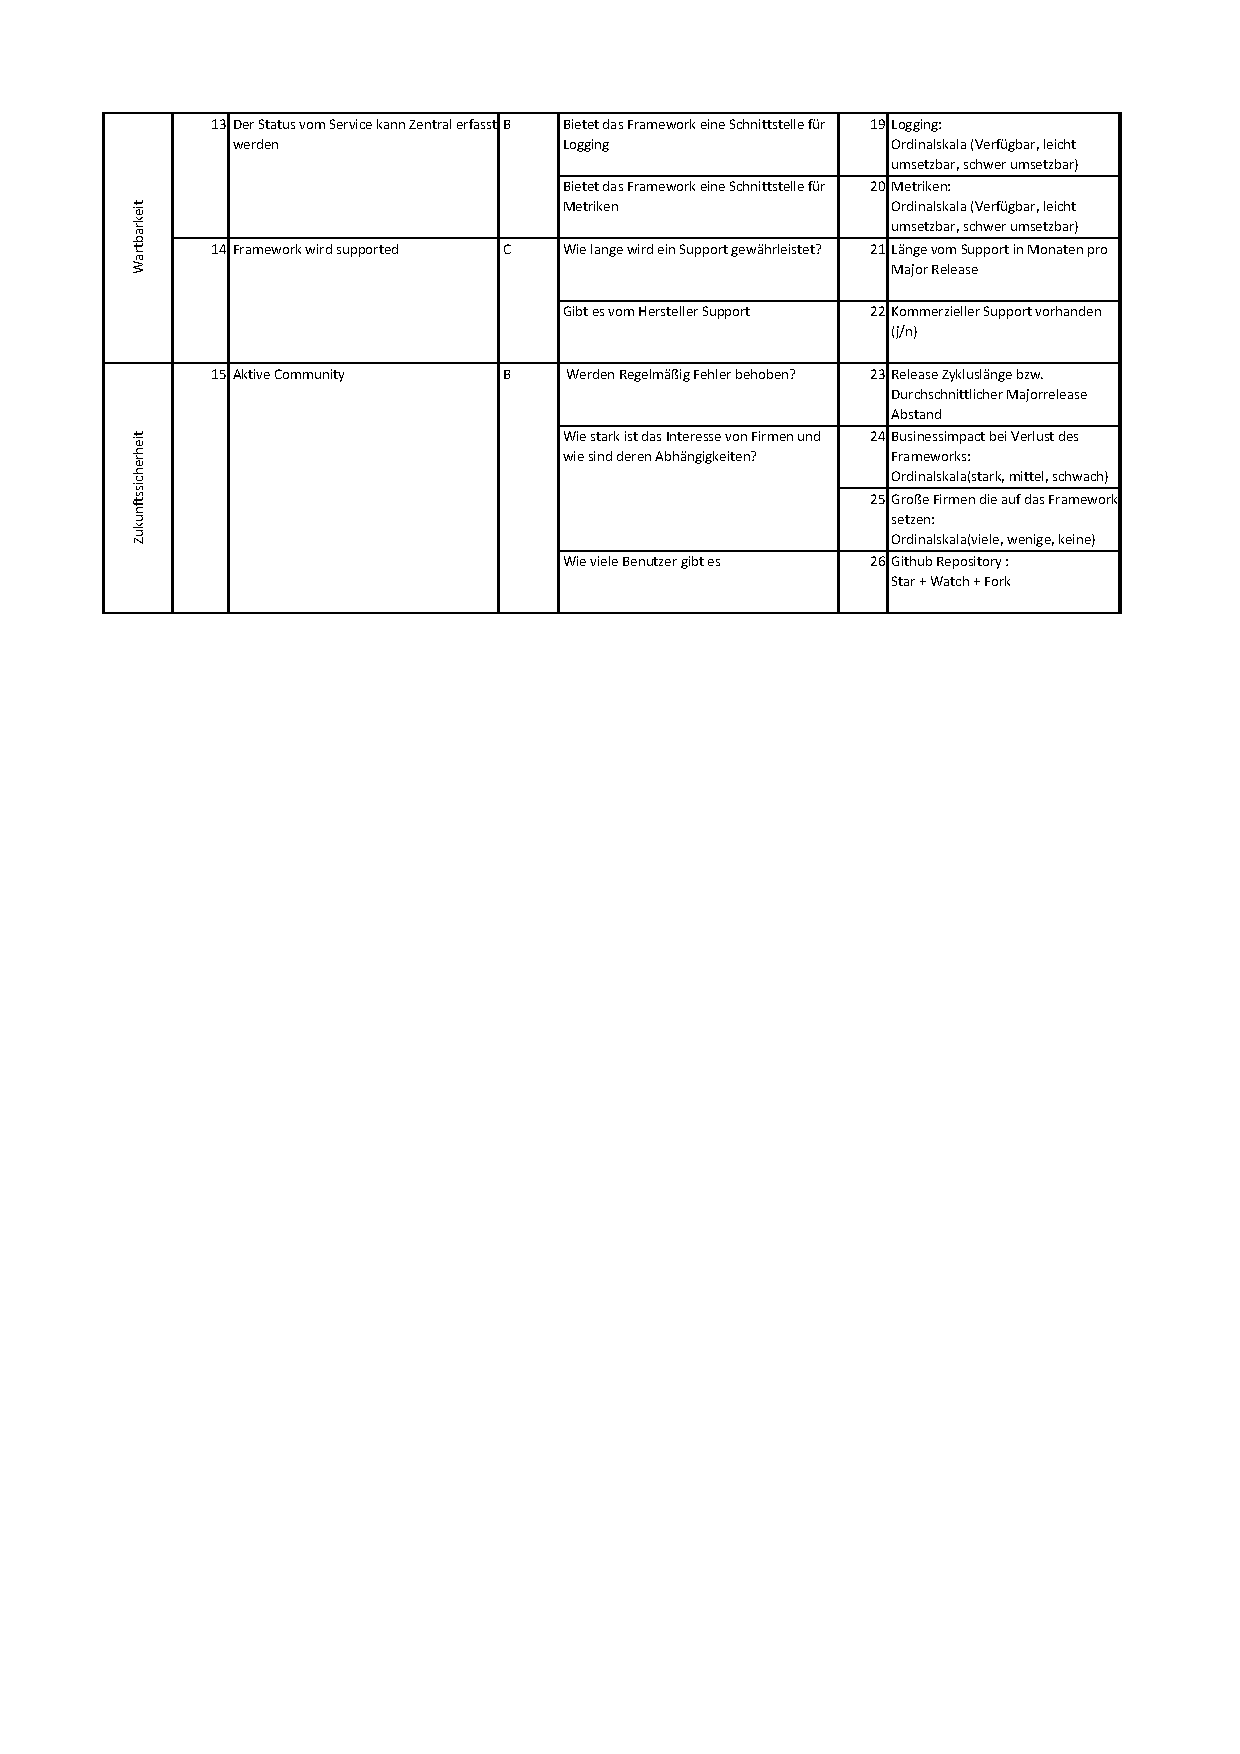
\includegraphics[width=\linewidth]{Bilder/GQM2.pdf}	\\
	\caption[Evaluation: Goal Question Metrik Tabelle]{Goal Question Metrik Ergebnis}
	\label{GQM}\\
\end{longtable}
\FloatBarrier

\subsubsection{Resümee Analysephase}
Die Basisanforderungen stellen eine gute Grundlage für die Wahl der Anforderungen da und beschleunigen somit die Analysephase. Dadurch konnte der \acl{QUT} schnell aufgebaut und priorisiert werden. Es bietet sich dabei an, dass der \ac{QUT} mit den Basisanforderungen vor dem Brainstorming für die Anforderungen vorbereitet ist und entsprechend angepasst wird.\\
Bei der Definition von Metriken fällt auf, dass viele qualitative Metriken, die Ordinalskalen, verwendet wurden. Dies lässt den Ursprung von \ac{MFEM} in der qualitativen Architekturbewertung erkennen. Aus Sicht des Autors bieten die Ordinalskalen einen guten Ansatz, um auch weiche Daten zu quantifizieren. Zusammen mit den weiteren Metriken kann das Framework so von allen Seiten betrachtet werden.\\
Wie sich der Einsatz der gefunden Metriken auswirkt, kommt aus dem den folgenden Phasen hervor.

\subsection{Evaluationsphase}

In der Evaluationsphase wird nun der Ablauf der Evaluation geplant und durchgeführt. Hierzu werden im nächsten Schritt Szenarien definiert.

\subsubsection{Evaluation definieren}

Die Evaluation wird in subjektiv und objektiv aufgeteilt. Für die subjektive Evaluation werden Szenarien definiert, die die Anforderungen bzw. Metriken untersuchen sollen.\\
\ac{MFEM} sieht hierzu die Definition eines Standard-Anwendungsfalls vor, der in mehrere Teile, den Szenarien, aufgeteilt wird. Hier wurde die Erstellung eines einfachen Daten-Service definiert, der sich mit dem Beispiel aus Kapitel \ref{Evaluation_definieren} deckt. Aus diesem Grund werden auch die Beispiel-Szenarien aus Kapitel \ref{Evaluation_definieren} übernommen und hier nur kurz zusammengefasst:

\begin{description}[leftmargin=!,labelwidth=\widthof{\bfseries Sz.3 Erweiterter Service}]
	\item[Sz.1 Installation] Installation der Sprache sowie des Frameworks und Einrichtung der Build-Tools
	\item[Sz.2 Einfacher Service] Programmierung eines einfachen "Hello World"-Services, inklusive Security
	\item[Sz.3 Erweiterter Service] Erweiterung des einfachen Services um ein Datenmodell (Aufgabenverwaltung)  
\end{description} 

Für die objektive Evaluation stehen nach \ac{MFEM} bereits Messgruppen fest. Diese umfassen die Messung an Artefakten, wie z.~B. dem Code, die Performance-Messung am lauffähigen Prototyp sowie der Recherche.\\
Um für die Messungen am laufenden Prototyp definierte Umstände zu haben, werden hier noch Anforderungsprofile benötigt. Dabei wurden folgende Profile für die Evaluation festgehalten:

\begin{table}[!h]
	\centering
	\begin{tabular}{p{1cm}p{4cm}p{2cm}p{2cm}p{4cm}}
		\textbf{Nr.} & \textbf{Typ} & \textbf{Parallele Verbindungen} & 
		\textbf{Dauer} & \textbf{Besonderheit} \\
		\hline
		1 	& Datenservice 			& 255	&	30s		& CRUD Operationen auf Datenbank  \\
		\hline
		2	& Einfacher Service		& 255 	&	30s		& Wenig rechenintensive Geschäftslogik   \\
		\hline
	\end{tabular}
	\caption[Anforderungsprofile]{Anforderungsprofile für die objektiven Evaluation am Prototyp}
	\label{AnforderungsprofileEval}
\end{table}

Insgesamt ergeben sich für den nächsten Schritt somit 6 Messgruppen, denen Metriken zugeordnet werden können.
Diese sind in Abbildung \ref{MessgruppenEval} nochmal zusammengefasst.

\image[MessgruppenEval.pdf]{MessgruppenEval}{Messgruppen für Evaluation}{Zusammenfassung aller Messgruppen für Evaluation}

\subsubsection{Metriken zuordnen}

Die Zuordnung der Metriken beginnt mit den Szenarios. Da diese zur subjektiven Evaluation gehören, werden nur weiche Daten erhoben. Im aktuellen Fall betrifft dies somit die mittels Ordinalskala erhobenen Metriken.

Da das Szenario 1 die Installation und Einrichtung übernimmt, wurden hier z.~B. Metriken der Anforderungen \enquote{Build-Tools} oder \enquote{Dependencieverwaltung} zugeordnet. Mit dem Szenario 2, dem einfachen Service, konnten die Standardformate und Security (\ac{JWT}) zugeordnet werden. Als letzte wurden dem Szenario 3, dem erweiterten Service, die Metriken für die \ac{REST}-Schnittstelle sowie Objektvalidierung zugeordnet. Zusätzlich wurden diesem Szenario, da es das Fortgeschrittenste ist, auch die Dokumentation und effiziente Programmierung zugeteilt.\\
Somit blieben am Ende des ersten Durchlaufs Metriken für Anforderungen wie z.~B. Logging, Service-Discovery und Circuit-Breaker-Pattern übrig. Aus diesem Grund mussten die Szenarios weiter verfeinert werden. Die Wahl fiel dabei auf das Szenario 2. Es sollte somit nicht nur ein "Hello World"-Service entstehen, sondern auch ein Service der bereits in der Infrastruktur funktioniert. Somit ließen sich auch die letzten Metriken zuordnen. 

Es ergibt sich somit die in Tabelle \ref{SzMetriken} gezeigte Zuordnung.  

\begin{longtable}{c}
	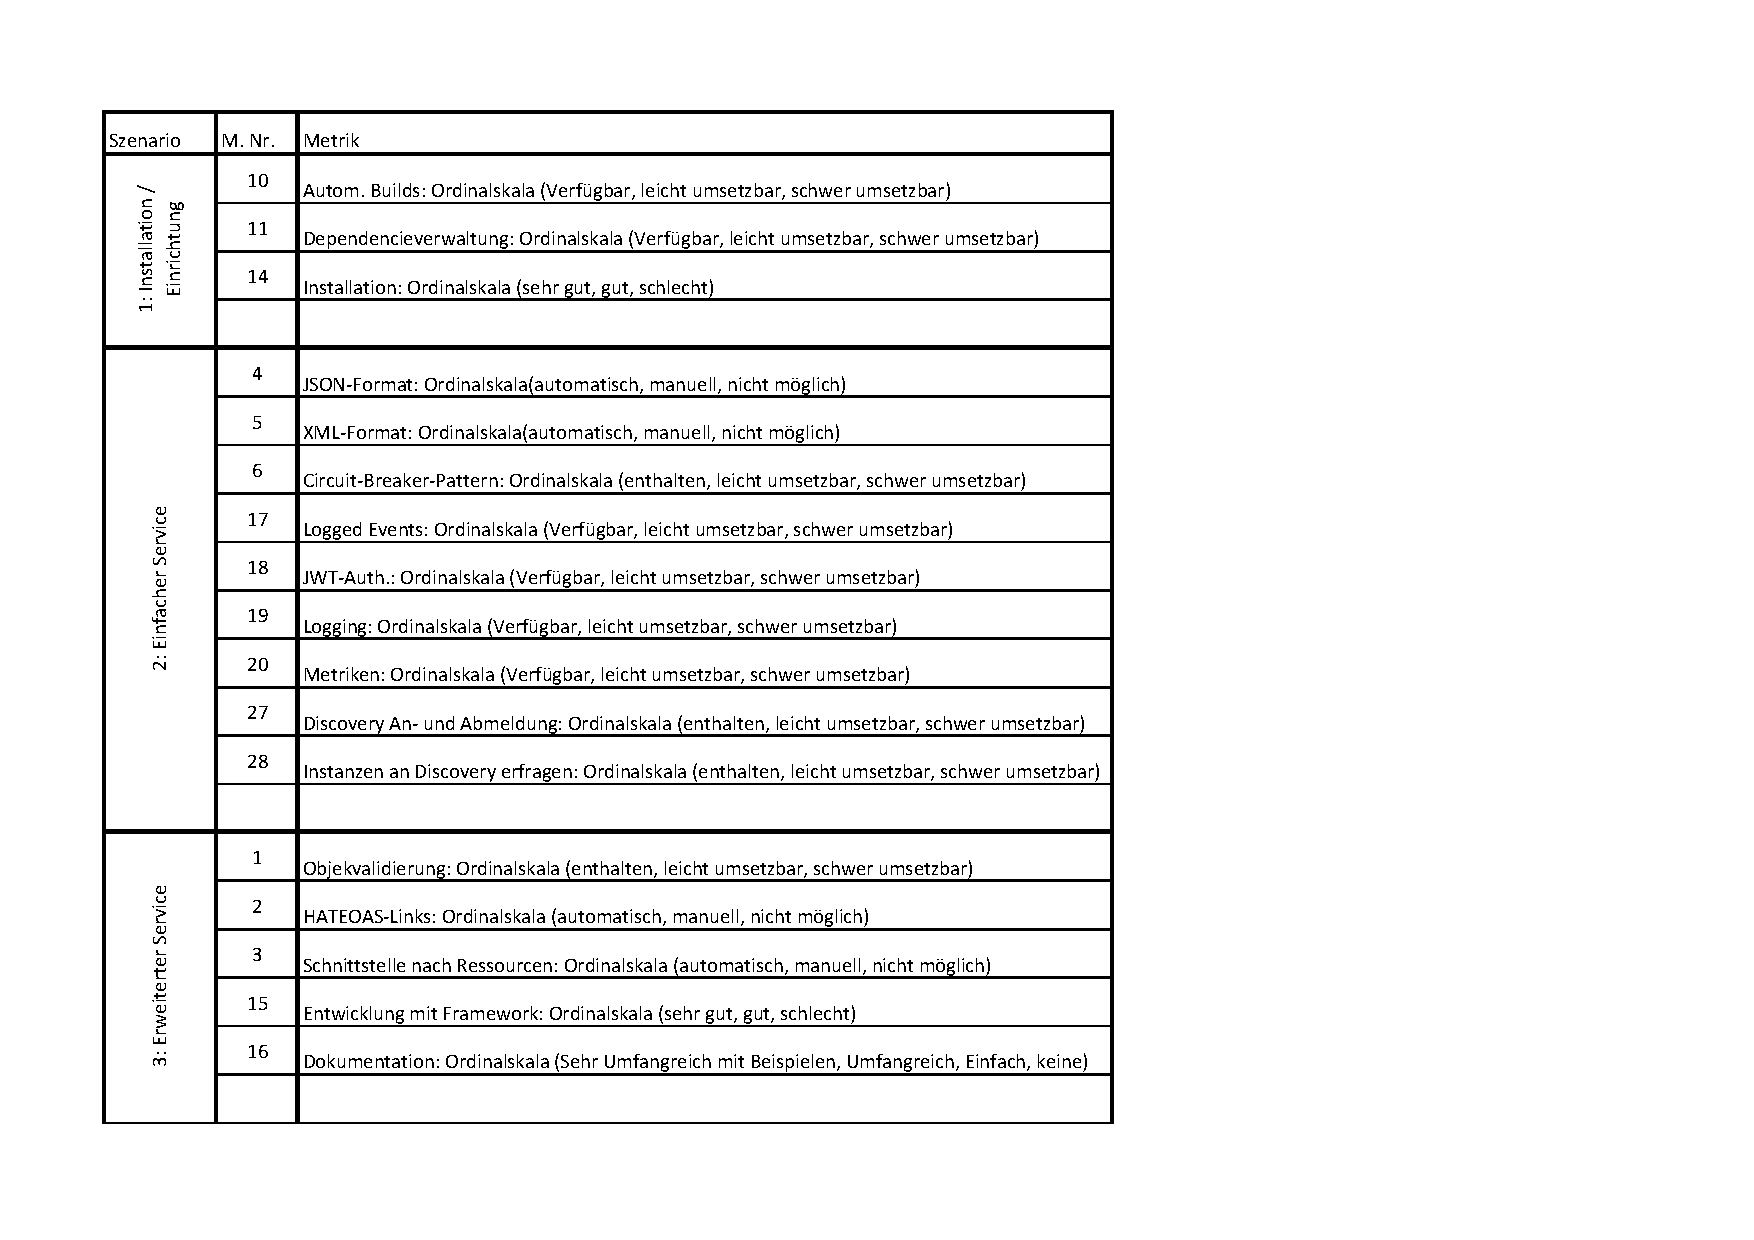
\includegraphics[width=\linewidth]{Bilder/SzMetriken.pdf} \\	
	\caption[Metriken Szenarios]{Szenarios: Zugeordnete Metriken}
	\label{SzMetriken}\\
\end{longtable}
\FloatBarrier

Da die objektiven Metriken sich nur an ihrem definierten Messpunkt erheben lassen, z.~B. kann der Durchsatz nur am lauffähigen Prototyp ermittelt werden, ließen sich diese einfach auf die 3 verbleibenden Messgruppen verteilen. 

Es ergibt sich somit die in Tabelle \ref{ObjekEvalMetriken} gezeigte Zuordnung. 

\begin{longtable}{c}
	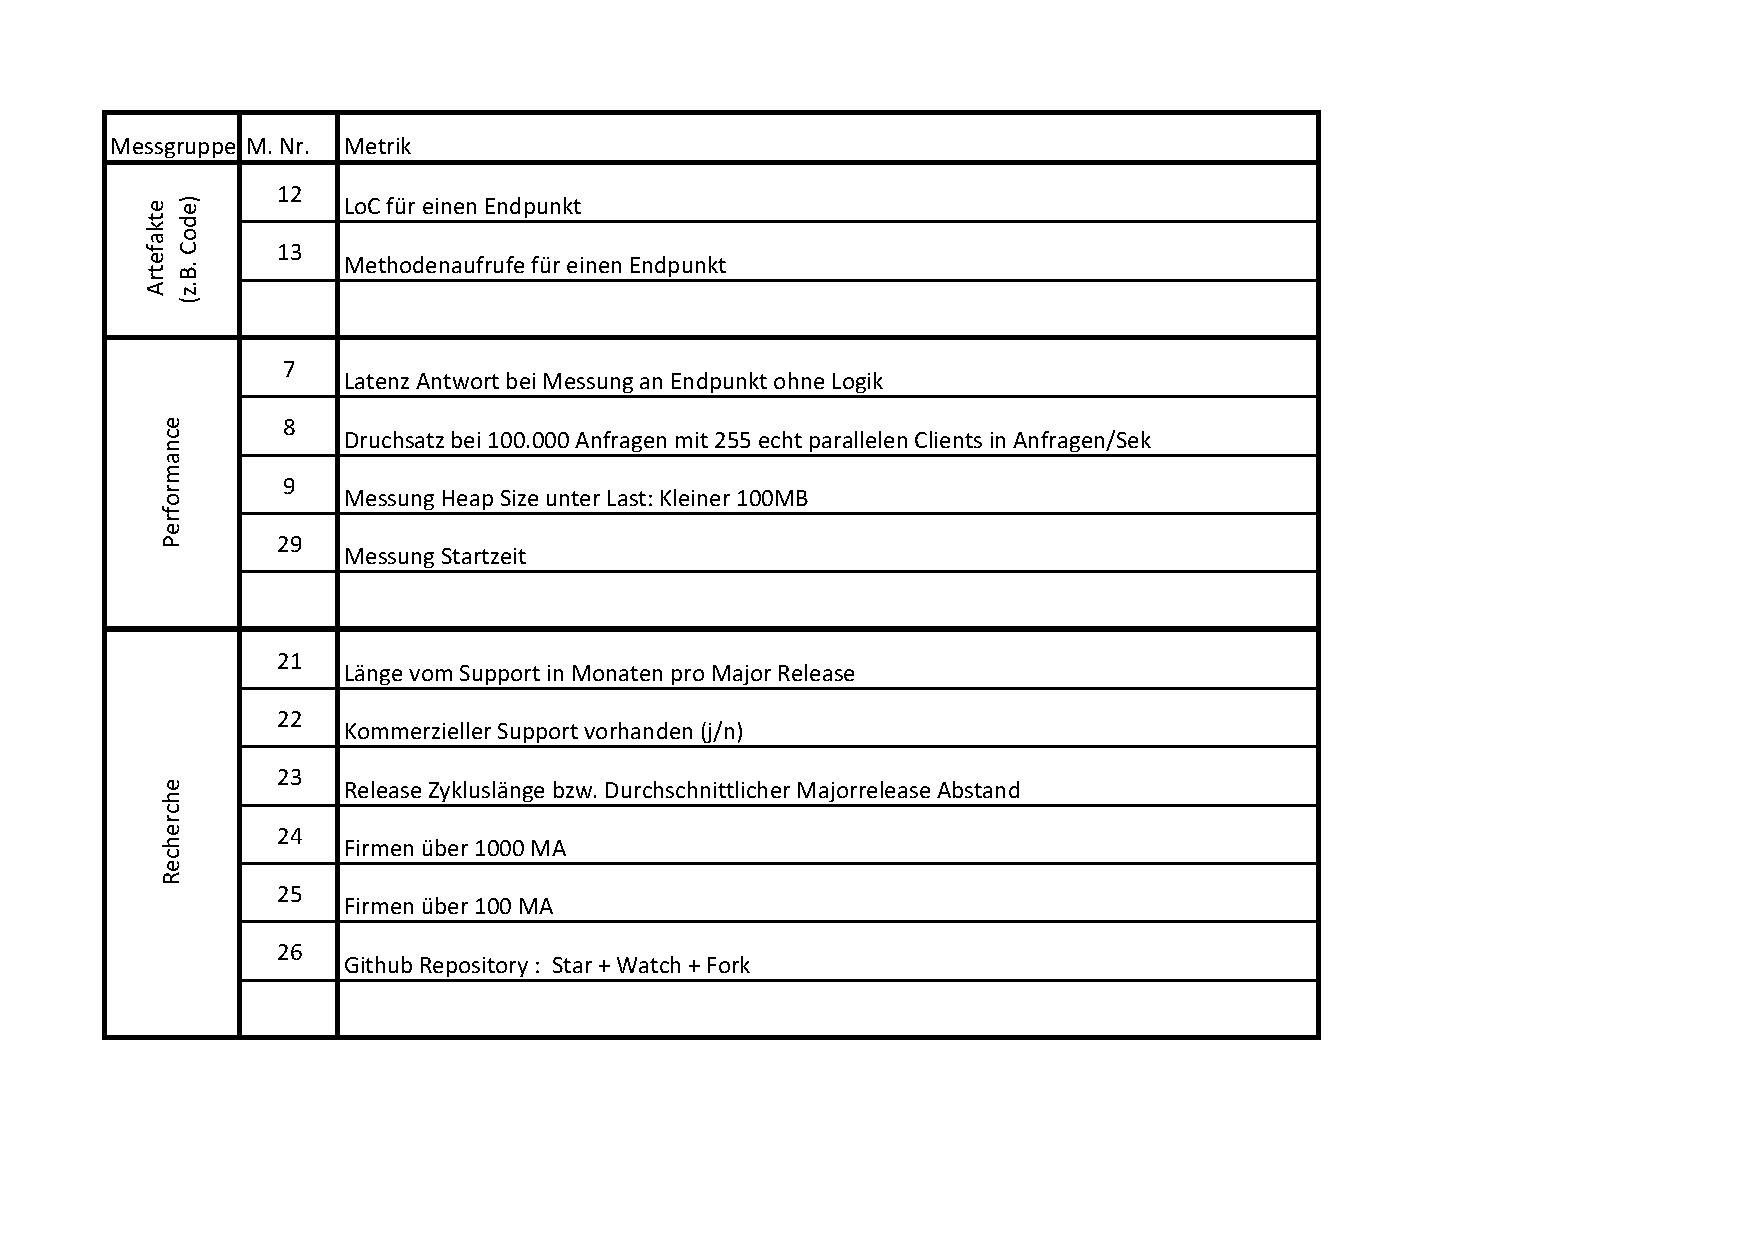
\includegraphics[width=\linewidth]{Bilder/ObjekEvalMetriken.pdf} \\	
	\caption[Metriken Objektive Evaluation]{Objektive Evaluation: Zugeordnete Metriken}
	\label{ObjekEvalMetriken}\\
\end{longtable}
\FloatBarrier

Da nun festgelegt ist, an welchem Punkt welche Daten erhoben werden, kann die Evaluation der Kandidaten durchgeführt werden.

\subsubsection{Evaluation durchführen: Spring Boot}

An dieser Stelle werden die Szenarien und Messungen an Spring Boot vorgenommen. Da es bei der Evaluation von \ac{MFEM} weniger um die konkrete Implementierung\footnote{
	Die gesamte Implementierung findet sich auf einem Github Repository mit der URL:\url{https://github.com/darenegade/SimpleSpringService}
} 
 geht, wird die Durchführung der einzelnen Messgruppen nur kurz beschrieben. Dabei werden markante Punkte hervorgehoben, sodass die Ergebnisse nachvollziehbar bleiben. 

\newparagraph{Szenario 1: Installation}
Mit Spring Boot wird Java als Programmiersprache benötigt. Die nötigen Installationsdateien lassen sich für jedes Betriebssystem bei Oracle\footnote{\url{http://www.oracle.com/technetwork/java}} beziehen.\\
Als Buildmanagement-Tools haben sich Gradle\footnote{\url{https://gradle.org}}  und Maven\footnote{\url{https://maven.apache.org}} etabliert. Beide sind für die Verwendung mit Spring gut geeignet. Und da keines augenscheinlich einen Vorzug aufweist, wurde Maven gewählt. Die Installation ist sehr einfach und es werden keine Vorkenntnisse benötigt. So konnten alle Metriken mit den bestmöglichen Werten bewertet werden.

\begin{longtable}{c}
	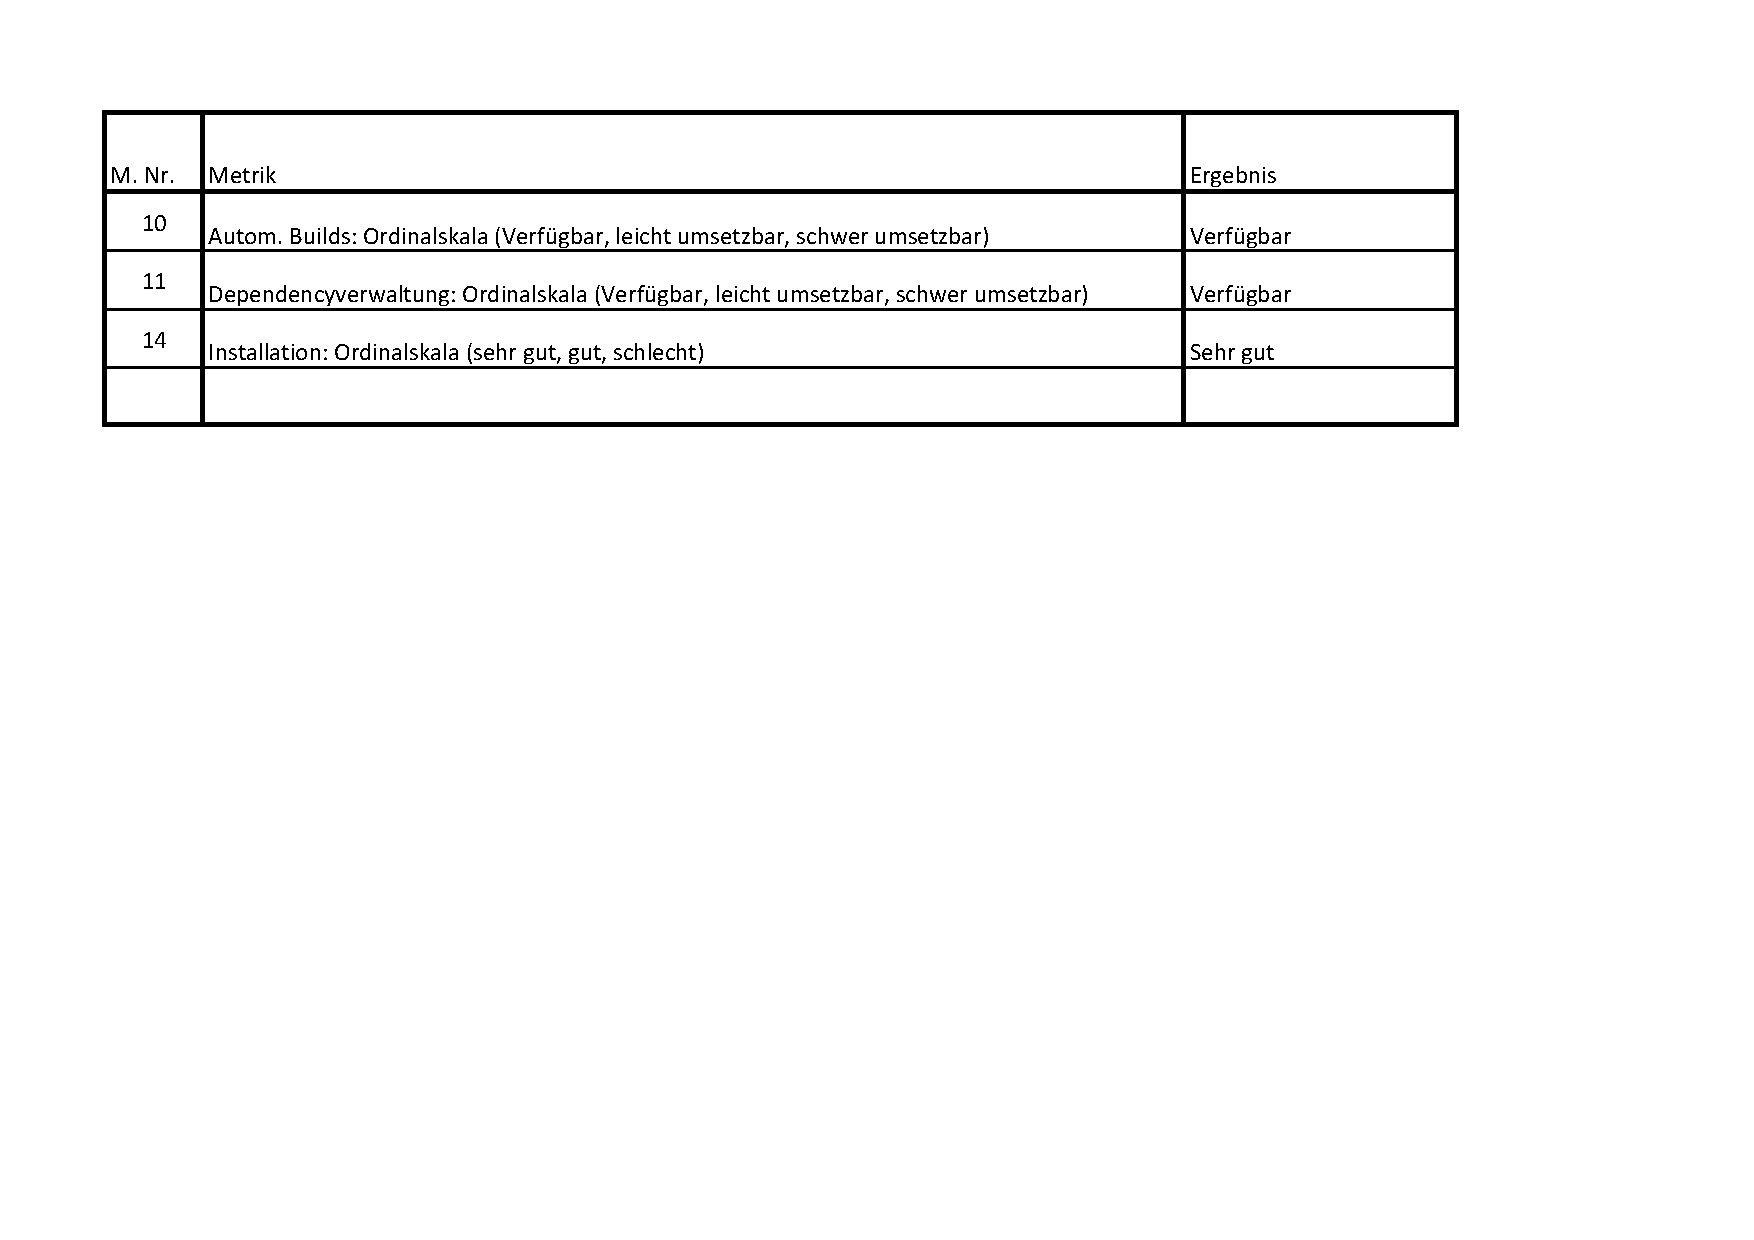
\includegraphics[width=\linewidth]{Bilder/Sz1ErgebnisSpring.pdf} \\	
	\caption[Szenario 1 Ergebnis Spring]{Ergebnis von Szenario 1 für Spring}
	\label{Sz1ErgebnisSpring}\\
\end{longtable}
\FloatBarrier

\newparagraph{Szenario 2: Einfacher Service}
Für die Erstellung eines neuen Projektes bietet Spring einen Initialisierungsservice\footnote{\url{http://start.spring.io}} an. Dieser lässt einen die nötigen Spring Module auswählen und das Projekt vorkonfigurieren. Als Ergebnis erhält man ein vollständig konfiguriertes Maven Projekt.
Dies macht den Einstieg sehr unkompliziert.

Auch die Implementierung eines "Hello-World"-Service ist mit Spring denkbar einfach. Das Listing \ref{SpringHello} zeigt was hierfür nötig ist. Daran sieht man sehr gut, dass die Einstiegshürde sehr gering ist. 
Mit \lstinline|@SpringBootApplication| werden die Standard-Spring\-konfigurationen aktiviert. So lässt sich anschließend über \lstinline|@RestController| und \lstinline|@PostMapping| der "Hello-World"-Endpunkt erstellen.
Mehr Konfiguration ist dabei nicht nötig, da Spring über die automatische Konfiguration die Parameter sowie den Rückgabewert der Methode erkennt und damit den Endpunkt anlegt. Auch die De- und Serialisierung in die Standardformate erfolgt automatisch und muss nicht manuell erstellt werden. Somit konnten diese Anforderungen mit \enquote{automatisch} bewertet werden. 

\begin{minipage}{\linewidth}
	\begin{lstlisting}[caption={"Hello-Word" in Spring},label=SpringHello,language=JAVA] 
		@SpringBootApplication
		@RestController
		@EnableEurekaClient
		public class Application {
		
			public static void main(String[] args) {
				SpringApplication.run(Application.class, args);
			}
			
			@PostMapping("/hello_service")
			public String helloService(@RequestBody Name name){
				return "Hello " + name.getName();
			}
		}
	\end{lstlisting}
\end{minipage}

Ähnlich mühelos gestaltet sich die Einrichtung der Service-Discovery Unterstützung. Mit der zusätzlichen Annotation \lstinline|@EnableEurekaClient| und einem Eintrag der Discovery-URL in der Datei \lstinline|application.properties| ist der Service für die Discovery konfiguriert. Die zugehörige Anforderung konnte somit bestmöglich bewertet werden. \\
Diese Kombination von Annotationen und einfachen Konfigurationen ist typisch für Spring Boot und konnte auf sämtliche weiteren Anforderungen angewendet werden. Das Ergebnis in Tabelle \ref{Sz2ErgebnisSpring} ist dementsprechend positiv.

\begin{longtable}{c}
	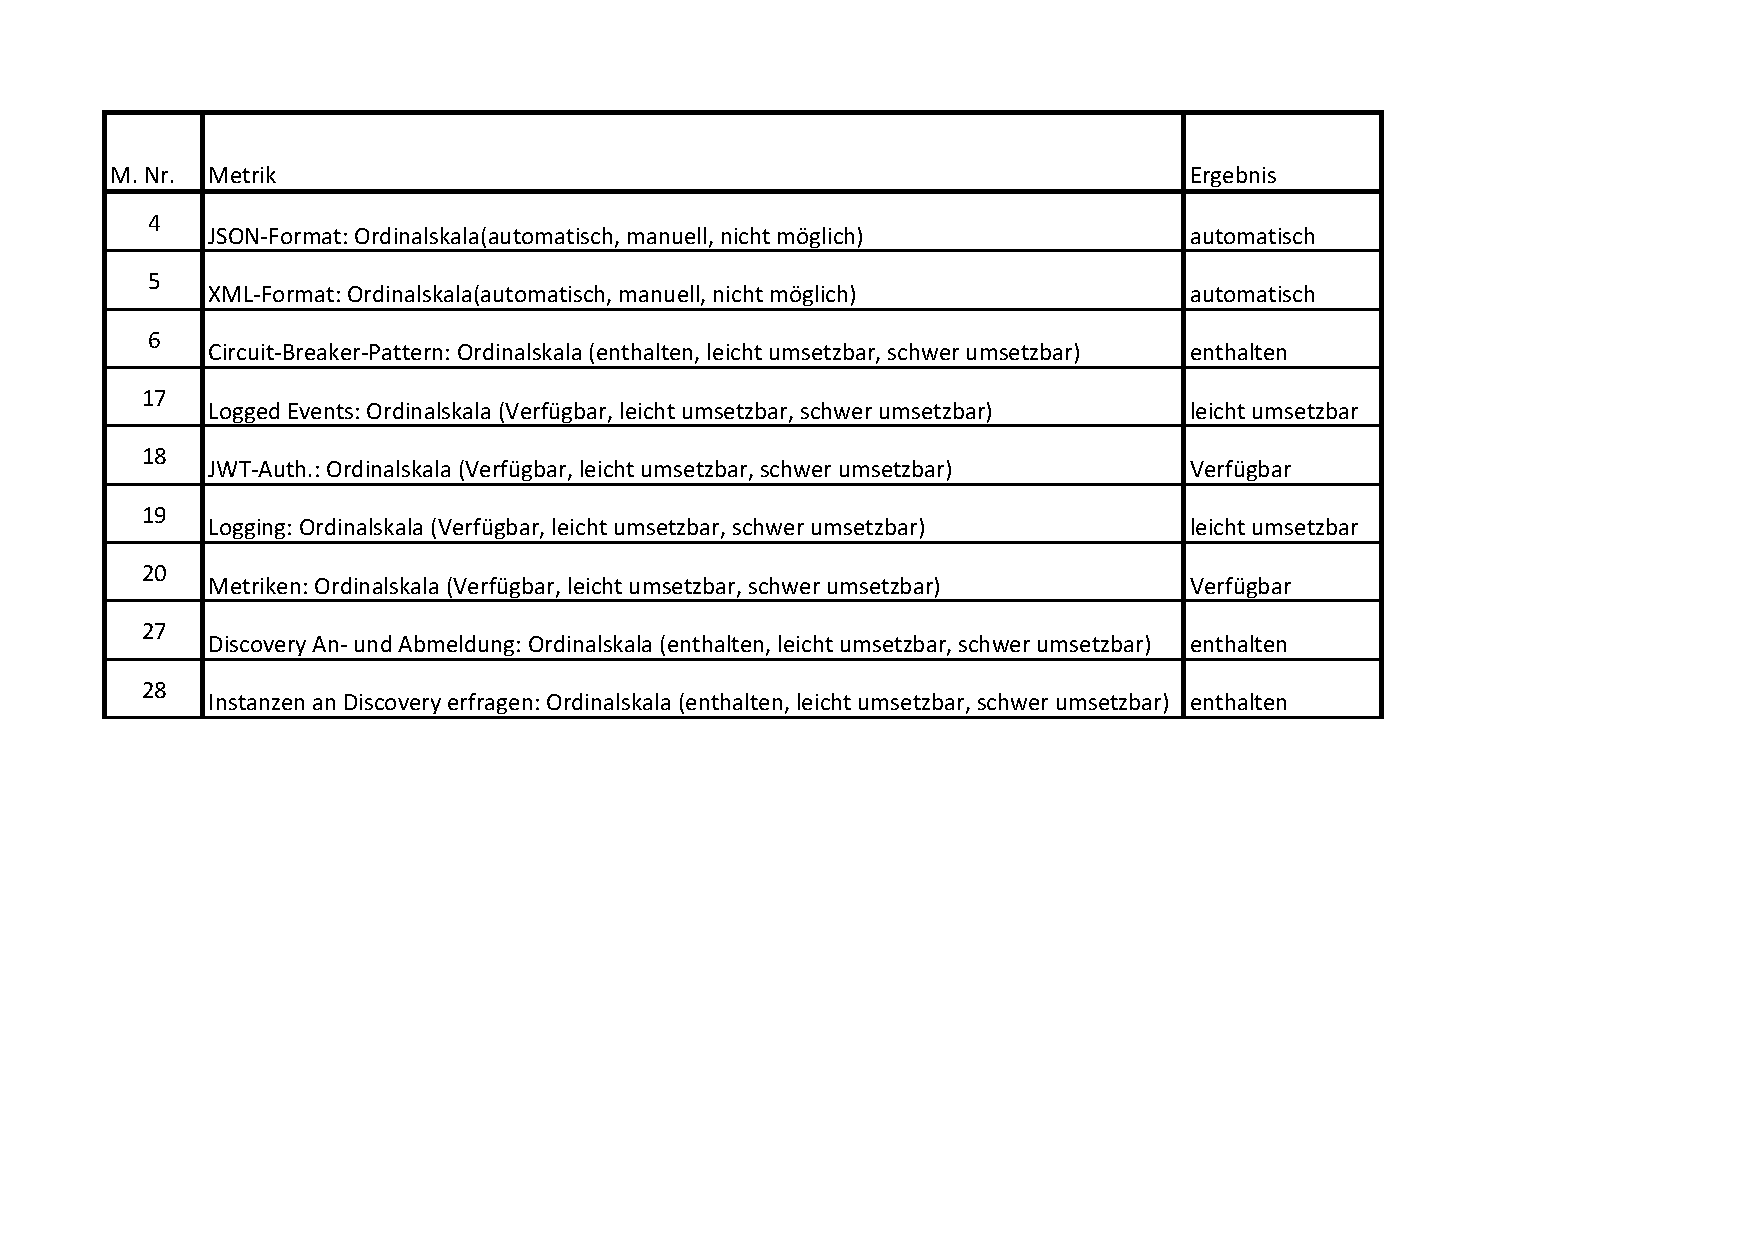
\includegraphics[width=\linewidth]{Bilder/Sz2ErgebnisSpring.pdf} \\	
	\caption[Szenario 2 Ergebnis Spring]{Ergebnis von Szenario 2 für Spring}
	\label{Sz2ErgebnisSpring}\\
\end{longtable}
\FloatBarrier

\newparagraph{Szenario 3: Erweiterter Service}
Das Szenario 3 sieht vor das Datenmodell für die Aufgabenverwaltung (Abbildung \ref{Datenmodell}) zu implementieren und über eine \ac{REST}-Schnittstelle nach außen anzubieten. Das Datenmodell wird dabei über die \ac{JPA} für Spring aufgebaut und die Konfiguration besteht somit auch aus Annotationen. Listing \ref{Department} zeigt dies als Beispiel für die Entität \enquote{Department}.

\begin{minipage}{\linewidth}
	\begin{lstlisting}[caption={Umsetzung der Entität \enquote{Department} mittels JPA},label=Department,language=JAVA] 
	@Entity
	public class Department extends BaseEntity{
	String name;
	
	@OneToOne
	@NotNull
	Employee head;
	
	@OneToMany
	Set<Employee> employees;
	
	//... Getter + Setter 
	}
	\end{lstlisting}
\end{minipage}

Die Besonderheit von Spring ist nun, dass mittels Spring-Data-Rest und dem in Listing \ref{DepRepo} gezeigten Code, die komplette \ac{REST}-Schnittstelle fertig konfiguriert ist. Das Repository-Interface muss lediglich als solches mit der Annotation \lstinline|@RepositoryRestResource| gekennzeichnet und von \lstinline|CrudRepository<T, ID>| abgeleitet werden, sodass Spring die Schnittstelle aufbauen kann. Diese ist vollständig nach Ressoucen aufgebaut und integriert in die Antworten automatisch \acs{HATEOAS} Links.

\begin{minipage}{\linewidth}
	\begin{lstlisting}[caption={Erstellung der REST-Schnittstelle für das \enquote{Department} über ein Interface},label=DepRepo,language=JAVA] 
	@RepositoryRestResource
	public interface DepartmentRepository extends 
									CrudRepository<Department, UUID> { 
	}
	\end{lstlisting}
\end{minipage}

Die Entwicklung eines Datenservice könnte somit kaum effizienter sein. Die automatische Konfiguration lässt sich auch anpassen. Hierzu bietet die Dokumentation detaillierte Beschreibungen und Code-Beispiele.\\
Somit konnte auch im 3. Szenario Spring sehr gut bewertet werden. Das Ergebnis ist in Tabelle \ref{Sz3ErgebnisSpring} zu sehen.

\begin{longtable}{c}
	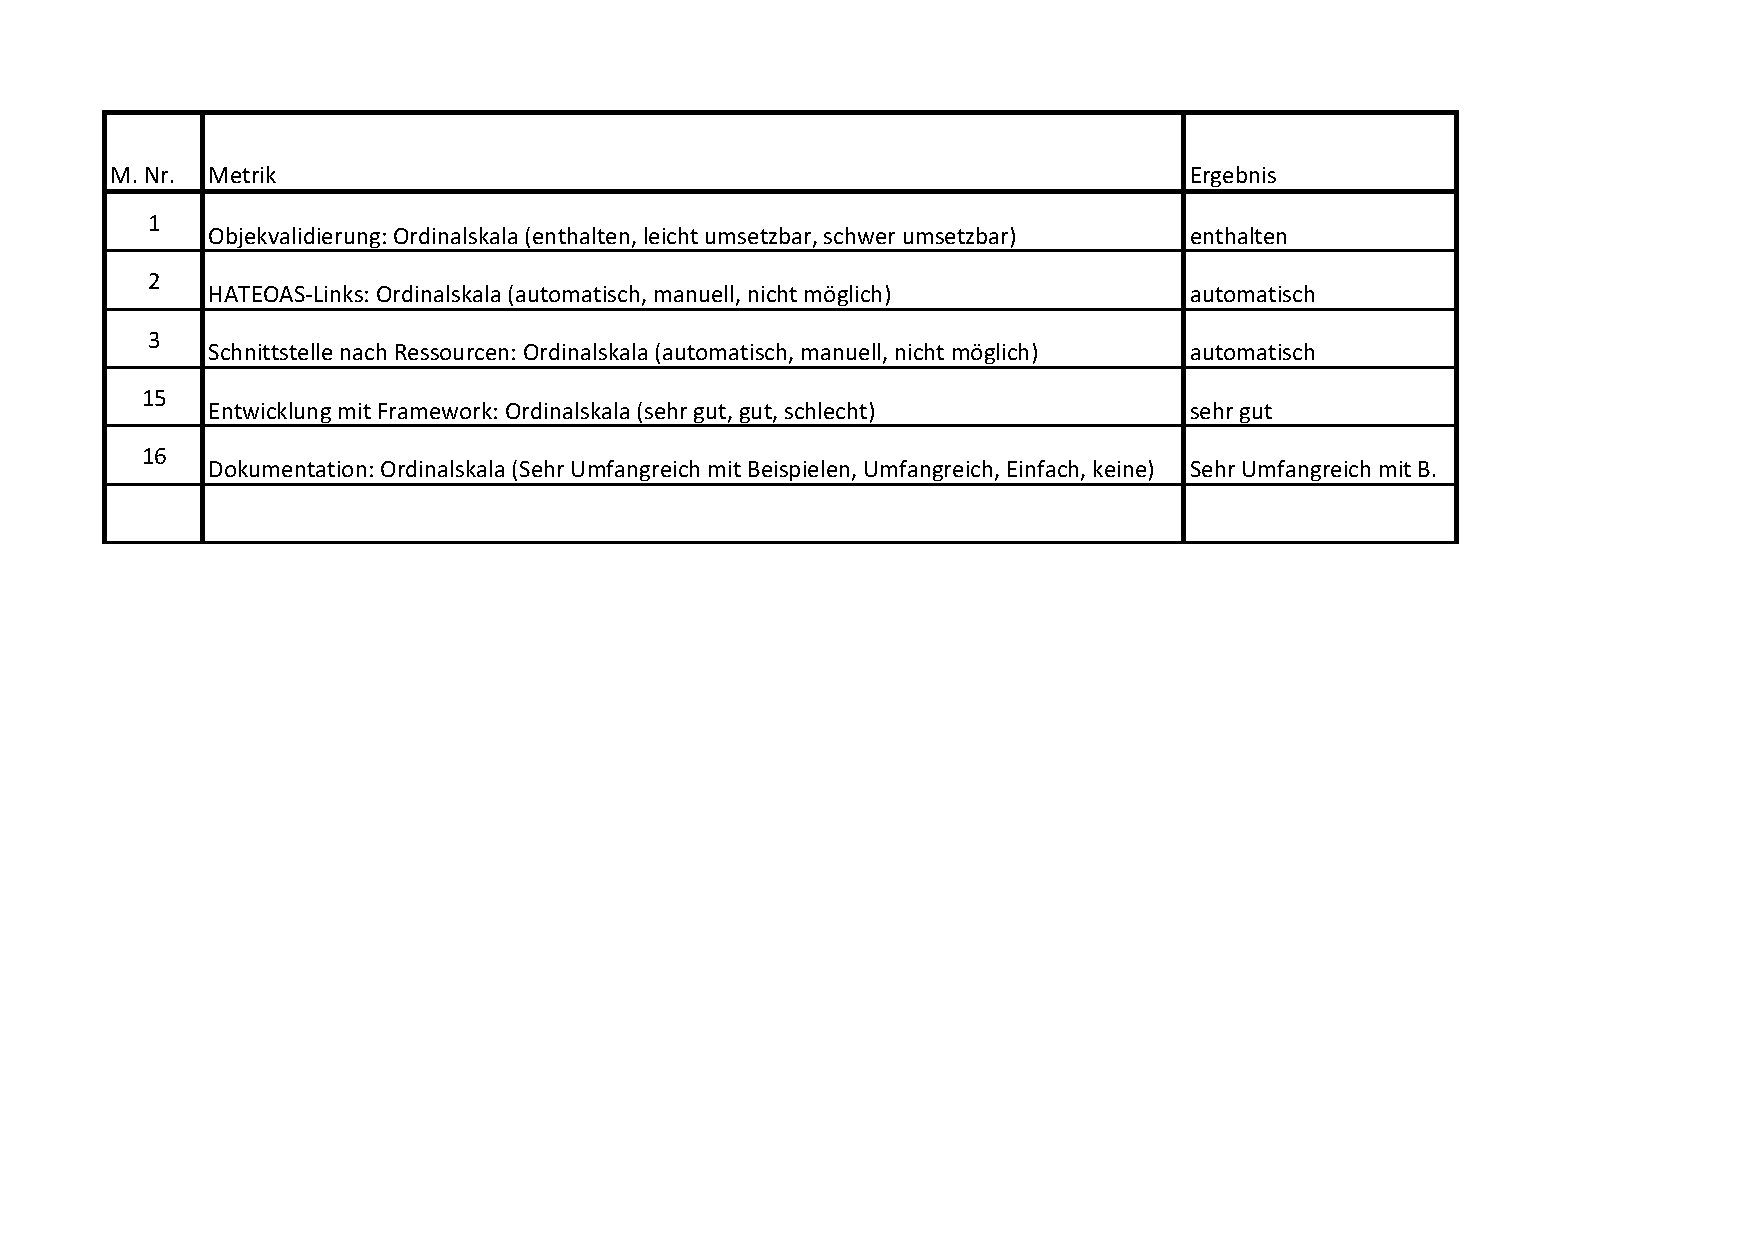
\includegraphics[width=\linewidth]{Bilder/Sz3ErgebnisSpring.pdf} \\	
	\caption[Szenario 3 Ergebnis Spring]{Ergebnis von Szenario 3 für Spring}
	\label{Sz3ErgebnisSpring}\\
\end{longtable}
\FloatBarrier

\newparagraph{Quantitative Evaluation}
Der aus dem 3. Szenario entstandene Prototyp kann nun für die Erhebung der harten Daten herangezogen werden. So wurden die \ac{LOC} und Methodenaufrufe für einen Endpunkt gemessen. Diese fallen, wie in Listing \ref{SpringHello} gezeigt, sehr gering aus. So bleibt die Codebasis auch bei vielen Endpunkten schlank und gut wartbar.\\
Des Weiteren wurden am lauffähigen Prototyp Performance Messungen durchgeführt. Hierzu wurde das Anforderungsprofil 2 aus der Tabelle \ref{AnforderungsprofileEval} auf den Prototyp angewendet und die entsprechenden Metriken, wie z.~B. Latenz, Durchsatz und Speicherverbrauch unter Last, gemessen\footnote{Für die Performance Messung wurde das Tool JMeter(\url{http://jmeter.apache.org}) eingesetzt und auf einem Laptop mit i7 2,3GHz Prozessor und 16GB DDR3 RAM durchgeführt.}. Die Anwendung des Anforderungsprofils 1 aus der Tabelle \ref{AnforderungsprofileEval} wurde für die Bestimmung der Metriken nicht benötigt und daher nicht weiter beachtet.

Die Recherche hat den Erwartungen entsprochen. Da Spring ein sehr etabliertes Framework ist, ist auch die Community sehr aktiv. Es werden regelmäßig Fehler behoben und neue Major-Releases veröffentlicht. Dies spiegelt auch die Akzeptanz bei großen Firmen wider. So setzen nach der offiziellen Webseite von Pivotal\footnote{\url{https://pivotal.io}}, der Organisation hinter dem Spring Framework, die 7 größten Banken oder die 9 größten Automanufakturen das Framework produktiv ein.

Die Ergebnisse der quantitativen Evaluation sind in der Tabelle \ref{QuantErgebnisSpring} festgehalten. Mit diesem Schritt wurde die Evaluation von dem Spring Framework beendet.  

\begin{longtable}{c}
	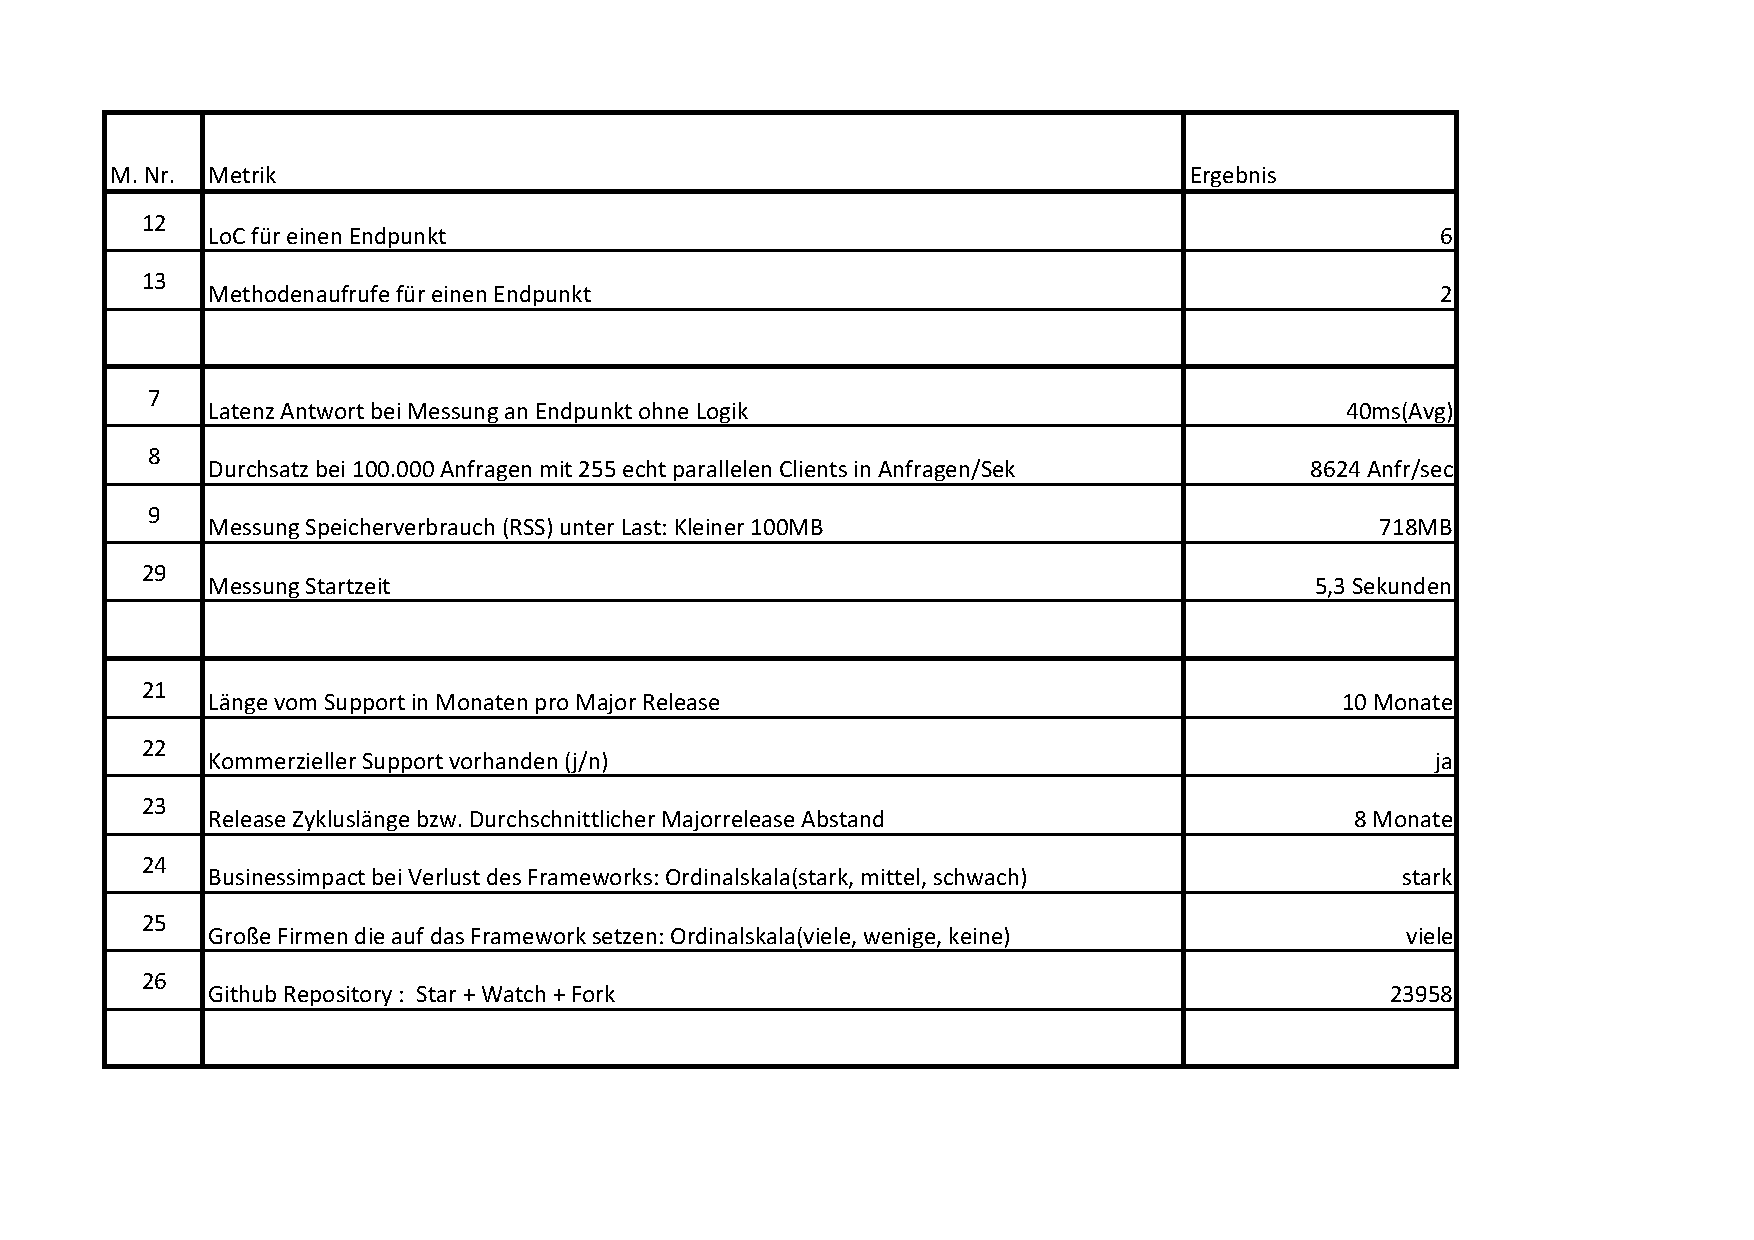
\includegraphics[width=\linewidth]{Bilder/ObjekEvalErgebnisSpring.pdf} \\	
	\caption[Quantitative Evaluation Ergebnis Spring]{Ergebnis der quantitativen Evaluation von Spring}
	\label{QuantErgebnisSpring}\\
\end{longtable}
\FloatBarrier

\subsubsection{Evaluation durchführen: Go-Kit}
Der zweite Kandidat für die Evaluation ist Go-Kit. Auch hier wird nicht auf die komplette Implementierung\footnote{
	Die gesamte Implementierung findet sich auf einem Github Repository mit der URL:\url{https://github.com/darenegade/SimpleGoKitService}
} 
eingegangen, sondern nur markante Punkte hervorgehoben. Dabei beginnt die Evaluation mit dem 1. Szenario.

\newparagraph{Szenario 1: Installation}
Go-Kit wird, wie der Name vermuten lässt, mit Go entwickelt. Daher ist die Installation von Go der erste Schritt. Hierzu lassen sich die Installationsdateien von der Webseite \url{golang.org} herunterladen und installieren.\\
Damit sind auch die essentiellen Tools für das Buildmanagement installiert. Diese sind z.~B. \lstinline|go get| für das Auflösen und Herunterladen von Abhängigkeiten (Dependencies) sowie \lstinline|go test| für das Ausführen von Unit-Tests.\\
Diese Befehle ersetzen aber kein vollständiges Buildmanagement-Tool, welches den kompletten Prozess steuert und die richtigen Abhängigkeiten auflöst\cite{GoDep2016}. So ist es notwendig den kompletten Prozess mittels Skript zu steuern und dabei Paketmanagement-Tools, wie Glide\footnote{\url{https://github.com/Masterminds/glide}}, zu nutzen.

Aus diesem Grund gab es für die Evaluation Abzüge bezüglich der Build-Tools. Die vollständige Bewertung ist in Tabelle \ref{Sz1ErgebnisGokit} festgehalten.

\begin{longtable}{c}
	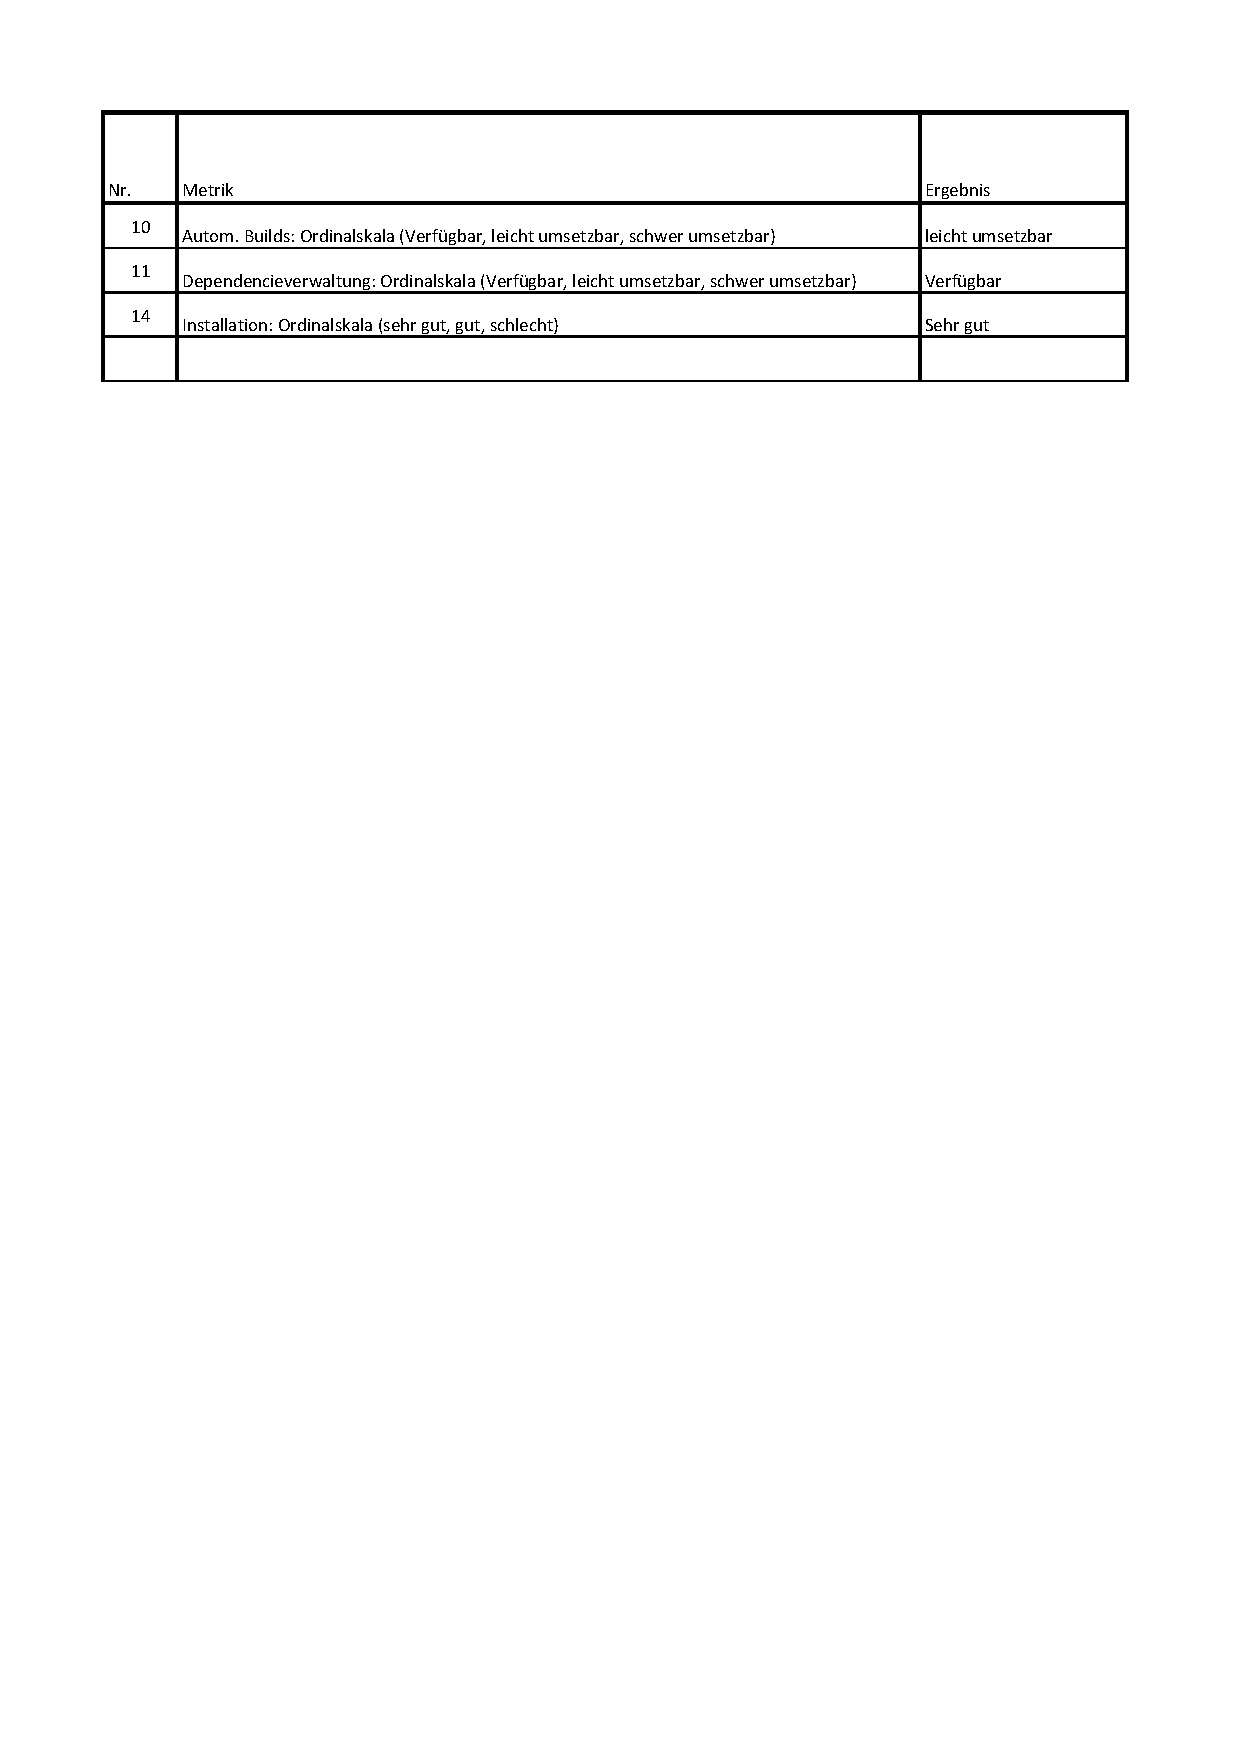
\includegraphics[width=\linewidth]{Bilder/Sz1ErgebnisGokit.pdf} \\	
	\caption[Szenario 1 Ergebnis GoKit]{Ergebnis von Szenario 1 für GoKIt}
	\label{Sz1ErgebnisGokit}\\
\end{longtable}
\FloatBarrier

\newparagraph{Szenario 2: Einfacher Service}
Im 2. Szenario wird ein einfacher "Hello World"-Service implementiert. Hierzu muss ein neues Projekt angelegt werden, welches im Workspace von Go, dem GoPath, erfolgen muss. Dabei ist das \lstinline|main.go| File der Einstiegspunkt einer jeden Go Applikation.\\
Die Implementierung des einfachen "Hello-Word"-Endpunktes ist in Listing \ref{HelloGo} dargestellt.

\begin{lstlisting}[caption={"Hello-Word" in Go-Kit},label=HelloGo,language=Golang] 
	func main() {
		logger := LOG.NewLogfmtLogger(os.Stdout)
		ctx := context.Background()
		svc := helloWorldService{}
		
		var helloWorldEndpoint endpoint.Endpoint
		helloWorldEndpoint = makeHelloWorldEndpoint(svc)
		
		helloWorldHandler := httptransport.NewServer(
			ctx, helloWorldEndpoint, 
			decodeHelloWorldRequest, encodeResponse,
			httptransport.ServerErrorLogger(logger),
		)
		
		http.Handle("/hello_service", helloWorldHandler)
		log.Fatal(http.ListenAndServe(":8080", nil))
	}
	
	type HelloWorldService interface {
		helloService(string) (string, error)
	}
	
	type helloWorldService struct{}
	
	func (helloWorldService) helloService(name string) (string, error) {
		return "Hello " + name, nil
	}
\end{lstlisting}

Dies zeigt sehr deutlich, dass die Erstellung eines Endpunktes relativ komplex ist. Es erfordert mehrere Konfigurationsschritte und muss vollständig manuell erfolgen, wobei der Ausschnitt nur ein Teil der gesamt nötigen Implementierung darstellt.\\
Auch ist die Verbindung zur Service Discovery an der Stelle noch nicht eingebaut. Go-Kit bietet für Eureka keine Unterstützung, sodass diese komplett eigenständig entwickelt werden muss. Da diese Anforderung mit \enquote{A} bewertet wurde und auch weitere Metriken ein mittelmäßiges Ergebnis aufweisen, könnte an dieser Stelle bereits über ein Abbruch der Evaluation diskutiert werden.\\
Im Sinne der Evaluation von \ac{MFEM} wurde entschieden, die Durchführung nicht abzubrechen. Das dabei entstanden Ergebnis ist in Tabelle \ref{Sz2ErgebnisGokit} zusammengefasst.

\begin{longtable}{c}
	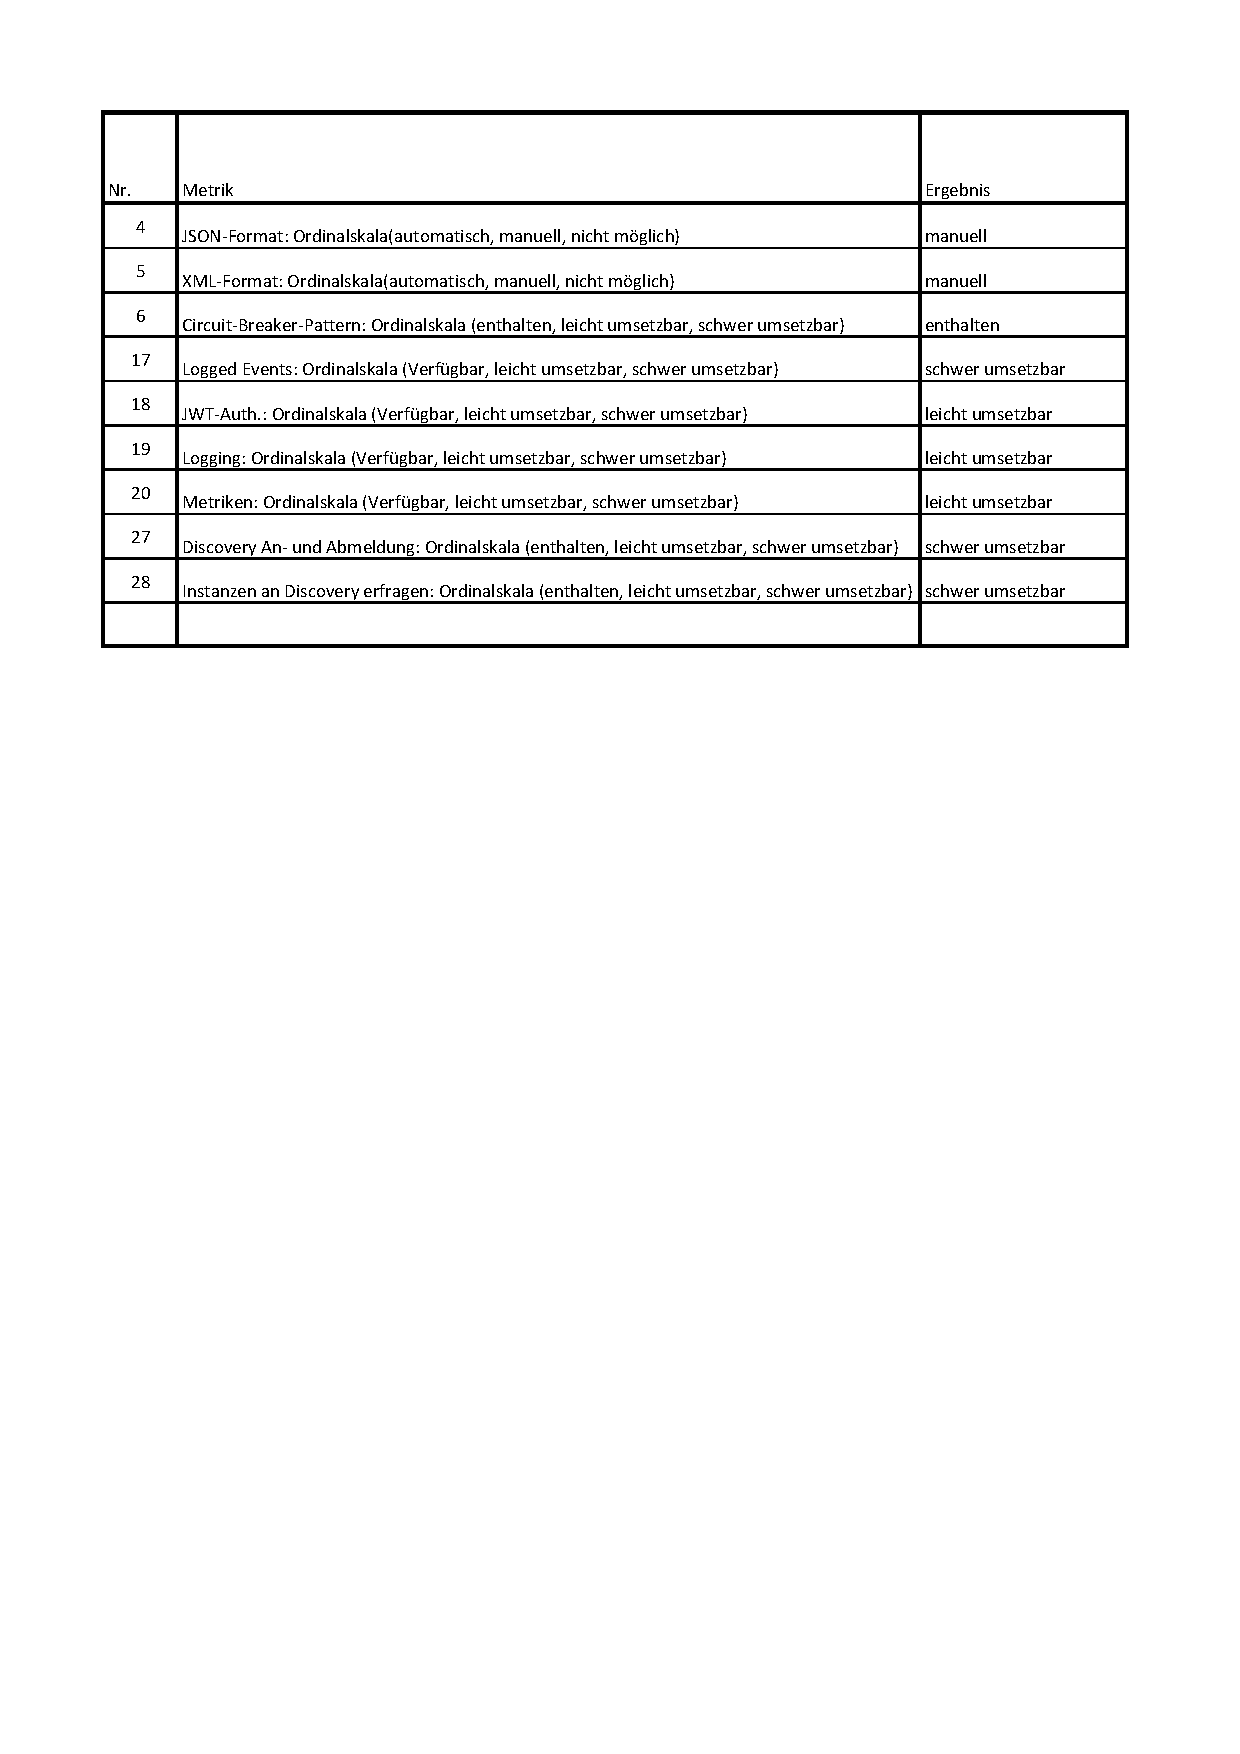
\includegraphics[width=\linewidth]{Bilder/Sz2ErgebnisGokit.pdf} \\	
	\caption[Szenario 2 Ergebnis GoKit]{Ergebnis von Szenario 2 für GoKIt}
	\label{Sz2ErgebnisGokit}\\
\end{longtable}
\FloatBarrier    

\newparagraph{Szenario 3: Erweiterter Service}
Auch beim erweiterten Service stößt man mit Go-Kit schnell an die Grenzen. Es bietet selber keine Unterstützung für eine Verbindung zu einer MySQL Datenbank. Um dies zu ermöglichen, wurde die Gorm\footnote{\url{http://jinzhu.me/gorm/}} Bibliothek mit aufgenommen. Es unterstützt die gängigsten Operationen auf einer Datenbank und verwaltet dabei das Datenschema.\\
Da Go-Kit somit nichts über die Datenbank weiß, kann es die \ac{REST}-Schnittstelle auch nicht nach Ressourcen aufbauen. Dies muss somit manuell erfolgen und für fast jede Operation muss ein eigener Endpunkt erstellt werden. Da dies analog zum Listing \ref{HelloGo} erfolgt, entsteht sehr viel \enquote{Boilerplate} Code, der die Entwicklung ineffizient macht. So wird der Code mit nur wenigen Endpunkten schnell unübersichtlich und schwer wartbar.\\
Bei der Umsetzung hilft die Dokumentation nur wenig. Sie enthält lediglich die Klassen sowie Packages und wenige einfache Beispiele. Tiefer greifende Erläuterungen sucht man vergebens.\\
Aus diesen Gründen ist die in Tabelle \ref{Sz3ErgebnisGokit} dargestellte Bewertung von Go-Kit für das 3. Szenario ernüchternd ausgefallen.

\begin{longtable}{c}
	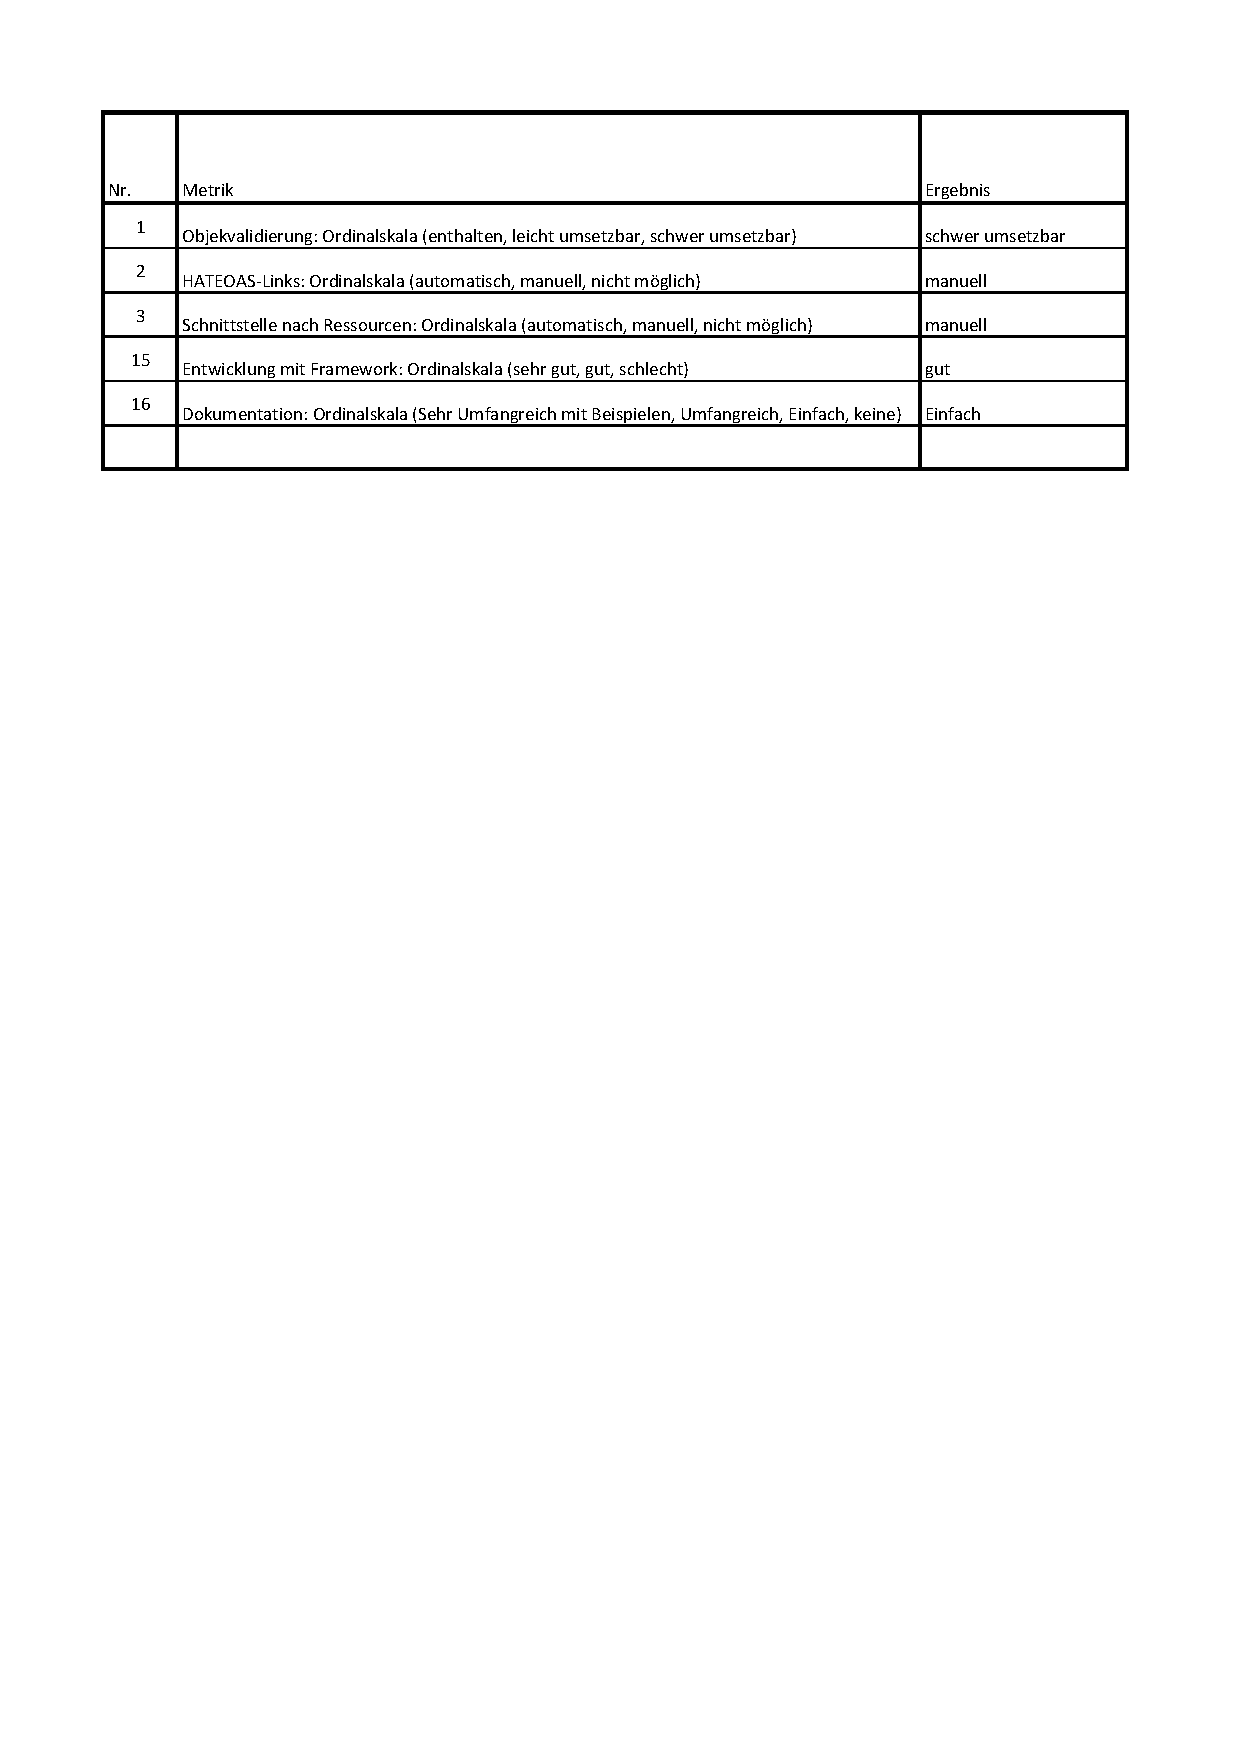
\includegraphics[width=\linewidth]{Bilder/Sz3ErgebnisGokit.pdf} \\	
	\caption[Szenario 3 Ergebnis GoKit]{Ergebnis von Szenario 3 für GoKIt}
	\label{Sz3ErgebnisGokit}\\
\end{longtable}
\FloatBarrier  

\newparagraph{Quantitative Evaluation}
Bei den Performance-Messungen konnte Go-Kit seine Stärken zeigen. Mit durchschnittlichen 9 Millisekunden Latenz kann der Service schnell Anfragen verarbeiten. So konnte er unter Last beachtliche 27.625 Anfragen/Sekunde beantworten und blieb dabei mit 31MB im Speicher sehr effizient\footnote{Für die Performance Messung wurde das Tool JMeter(\url{http://jmeter.apache.org}) eingesetzt und auf einem Laptop mit i7 2,3GHz Prozessor und 16GB DDR3 RAM durchgeführt.}.

Die Recherche bestätigte jedoch das bisher relativ schlechte Ergebnis. Obwohl das Framework auf der offiziellen Webseite als produktionsreif vermarktet wird\cite{GoKitFAQ2017}, steht es derzeit noch in Entwicklung und ist aktuell in der Version $0.3$ veröffentlicht. Somit gibt es zur Zeit weder einen offiziellen Support noch setzen, zu Recht, große Firmen auf dieses Framework.

Das Ergebnis der Quantitativen Evaluation ist in Tabelle \ref{QuantErgebnisGokit} dargestellt.  

\begin{longtable}{c}
	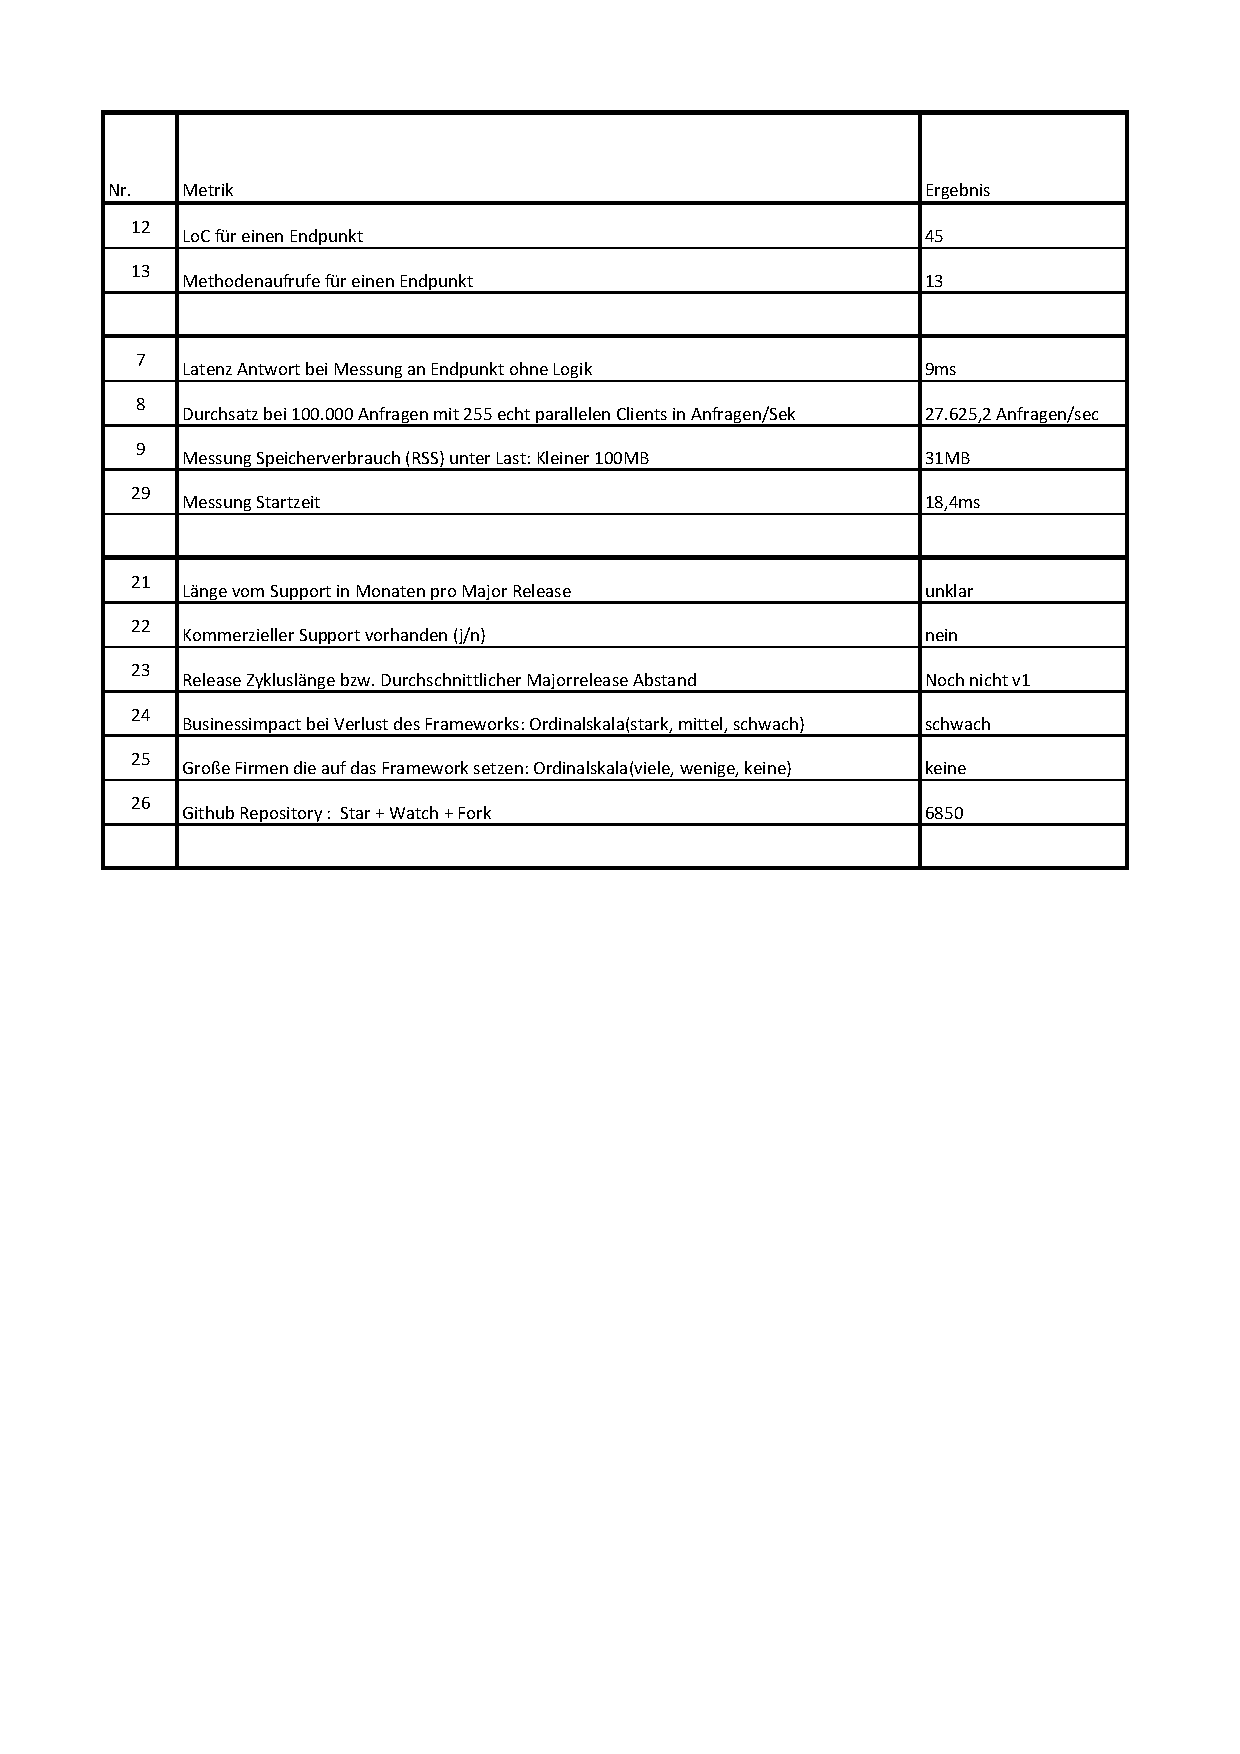
\includegraphics[width=\linewidth]{Bilder/ObjekEvalErgebnisGokit.pdf} \\	
	\caption[Quantitative Evaluation Ergebnis Go-Kit]{Ergebnis der quantitativen Evaluation von Go-Kit}
	\label{QuantErgebnisGokit}\\
\end{longtable}
\FloatBarrier

\subsubsection{Resümee Evaluationsphase}

Die Evaluationsphase ist die längste Phase von \ac{MFEM}. So hat die praktische Umsetzung der Szenarien und Messungen sowie die Einarbeitung in das Framework bei beiden Kandidaten eine Woche betragen. Aus diesem Grund ist es wichtig, bei der Ermittlung der Metriken auf die Prioritäten der Anforderungen zu achten. Wie bei der Evaluation von Go-Kit zu sehen war, hätte schon das Ergebnis des 2. Szenarios zu einem Abbruch führen können.\\
Durch die genaue Definition der Szenarien mit den zugehörigen Metriken erfolgt die Durchführung der Evaluation zudem sehr zielgerichtet. Mit etwas Disziplin kann so eine ausschweifende Entwicklung verhindert und somit der Zeitaufwand weitestgehend verkürzt werden. Hierzu sollten, wie von \ac{MFEM} vorgesehen, die Szenarien möglichst genau definiert werden.\\
Der Kreislauf zur Definition von Szenarien und der Zuordnung von Metriken hat sich in dieser Phase bewährt. So konnten keine Metriken übersehen und die Szenarien verfeinert werden.    

\subsection{Abschlussphase}

In der Abschlussphase werden die Ergebnisse aus der Evaluation aufbereitet und präsentiert. Aufgrund der Fülle von Anforderungen und erhobene Daten, wird dies hier nur exemplarisch an einer Qualitätskategorie für ein Framework durchgeführt. Die Auswertung der Restlichen erfolgt analog und findet sich als Excel Tabelle in den jeweiligen Github-Repositories sowie auf der beigelegten Daten-CD.

Die Aufbereitung der erhobenen Daten wird mit der komplexen Auswertung erfolgen. Die Abbildung \ref{AuswSpringWart} zeigt den kompletten Prozess.\\

\image[AuswertungSpringWartbarkeit.pdf][width=0.9\linewidth]{AuswSpringWart}{Auswertung Spring Wartbarkeit}{Auswertung und Zusammenführung aller Daten für die Qualitätskategorie \enquote{Wartbarkeit} am Beispiel Spring}

So wurden im ersten Schritt die ermittelten Ergebnisse auf einen Wert zwischen 0 und 1 normalisiert. Für die dreistufigen Ordinalskalen ergeben sich 3 mögliche Werte: $1$ für den höchsten, $0,5$ für den mittleren und $0$ für den niedrigsten Wert.\\
Bei den quantitativen Daten wird die prozentuale Abweichung zum Zielwert für die Normalisierung hergenommen. So ergab sich für die Supportlänge, mit einem Ergebnis von 10 und einem Zielwert von 12, ein Wert von $0,83$.
Die Erfüllung einer Ja/Nein-Frage kann wie eine zweistufige Ordinalskala angesehen werden. So wurde der vorhandene Support mit 1 normalisiert.\\
Nachdem die einzelnen Werte für eine Anforderung aufsummiert wurden, kann der prozentuale Erfüllungsgrad bestimmt werden. Bei 2 Anforderungen würde ein Wert von 2 einer vollen Erfüllung (100\%) entsprechen. Mit einem Wert von $1,5$ ergibt sich so ein Erfüllungsgrad von $87,5\%$.\\
Anhand der Prioritäten werden die Gewichte für die Zusammenführung der Anforderungen ermittelt. Eine mit \enquote{A} bewertete Anforderung geht vollständig in das Ergebnis über. Die Priorität \enquote{B} zählt zur Hälfte und \enquote{C} nur ein Viertel. So ergibt sich das Gesamtergebnis von $88,83\%$ für die Wartbarkeit von Spring.

Nachdem alle Ergebnisse aller Qualitätskategorien für Spring und Go-Kit mit diesem Schema ausgewertet wurden, konnte das Netzdiagramm erstellt werden. Abbildung \ref{FitnessVergleich} zeigt das Gesamtergebnis von Spring und Go-Kit in einer Grafik. 

\image[FitnessVergleich.pdf][width=0.9\linewidth]{FitnessVergleich}{Gesamtergebnis von Spring und Go-Kit}{Gesamtergebnis von Spring und Go-Kit als Netzdiagramm}
  
Das Gesamtergebnis macht die Überlegenheit von Spring deutlich. In nahezu jeder Kategorie hat es einen Vollausschlag. Lediglich bei der Performance kann Go-Kit Punkten. Aufgrund des miserablen restlichen Ergebnisses, wird jedoch auch dann von einem Einsatz im produktiven Umfeld abgeraten, falls die Geschwindigkeit ein maßgeblicher Faktor ist.\\
Der Einsatz von Spring ist dagegen sehr empfehlenswert, was der Erfolg und die weite Verbreitung des Frameworks zeigt.   

\subsubsection{Resümee Abschlussphase}

Die Auswertung der Daten ist sehr einfach und liefert ein ansehnliches Gesamtergebnis. Es kann dabei nur für sich stehen oder auch im Vergleich zu anderen Frameworks gut hergenommen werden, was die Abbildung \ref{FitnessVergleich} sehr gut zeigt. Auf dieser Basis kann schnell ein guter Überblick gewonnen werden, mittels dessen weitere Diskussionen durchgeführt oder Entscheidungen getroffen werden können.

\subsection{Gesamtauswertung \ac*{MFEM}}

Zusammenfassend kann gesagt werden, dass \ac{MFEM} seinen Zweck erfüllt. Die Diskrepanz, die bei der Wahl der Kandidaten eine Anforderung war, hat sich in den Ergebnissen widergespiegelt. So wurde trivialerweise ein gutes Framework äußerst positiv und ein unausgereiftes Framework negativ bewertet. Hierzu wurden, bis auf wenige Ausnahmen, nur die Basisanforderungen genutzt. So kann auch gesagt werden, dass diese bereits eine gute Grundlage für eine Bewertung darstellen.\\
Sämtliche Anforderungen lassen sich durch die Analysephase an die jeweilige Situation anpassen oder erweitern, sodass die Methode flexibel bleibt. Wie hier gezeigt wurde, entsteht so schnell eine Vielzahl an Anforderungen. Dazu bietet der Quality Utility Tree einen guten Ansatz, um den Überblick zu behalten und sich nicht in Feinheiten zu verlieren.\\
Die erste Hürde stellt die Wahl der passenden Metriken dar. Dies war auch bei dieser Evaluation durchaus eine Herausforderung. Auch wenn hier bis zuletzt kein Patentrezept für die Wahl der bestmöglichen Metriken ausgestellt werden kann, stellt die \ac{GQM} Methode einen guten Top-Down Ansatz dar, um dies zu unterstützen.

Bis zur Evaluationsphase, und selbst dort erst im letzten Schritt, spielt das eigentlich zu testende Framework keine Rolle. Dadurch bleibt die Methode sprachunabhängig und verkürzt sich bei mehrfacher Anwendung an verschiedenen Frameworks. Dieser Gewinn ist jedoch nur marginal, da die Durchführung der Evaluation am Framework den größten Zeitaufwand einnimmt. Hierzu bietet die Methode mit den Szenarien einen guten Ansatz, um den verhältnismäßig langen Prozess zumindest zielgerichtet zu gestalten. Wie sich gezeigt hat, kann durch die Priorisierung auch ein schneller Abbruch zustande kommen. So wird wenigstens nicht unnötig Zeit in einen negativen Kandidaten gesteckt.\\
Einzig die Abbruchbedingung wird von \ac{MFEM} nicht vorgegeben und sollte vor der Durchführung definiert werden. Eine Bedingung im Zusammenhang mit den Prioritäten ist hierfür prädestiniert.

Das mittels Netzdiagramm dargestellte Gesamtergebnis bietet einen sehr guten und schnellen Überblick über das Ergebnis. So kann der Architekt auch vor nicht allzu technisch versierten Entscheidungsträgern seine Wahl anschaulich begründen, ohne zu tief ins Detail gehen zu müssen.     












